\documentclass[12pt]{article}
\usepackage{mathbbold}
\textwidth=16.5cm \textheight=24cm \headheight=0cm \headsep=0cm
\usepackage{CJK}
\usepackage{cite}
\usepackage{ulem}
\usepackage{graphicx}
\usepackage{epstopdf}
\topmargin=-1cm
\oddsidemargin=0pt \evensidemargin=0pt
%\topmargin=-2cm

\usepackage{mathrsfs}
\usepackage{titlesec}
\usepackage{xcolor}
\usepackage{amssymb}
\usepackage{amsmath}
\usepackage{amsfonts}
\usepackage{cases}
\renewcommand{\baselinestretch}{1.8}


% 重定义字体命令
\newcommand{\song}{\CJKfamily{song}}    % 宋体   (Windows自带simsun.ttf)
\newcommand{\fs}{\CJKfamily{fs}}        % 仿宋体 (华天字库htfs.ttf)
\newcommand{\kai}{\CJKfamily{kai}}      % 楷体   (华天字库htkai.ttf)
\newcommand{\hei}{\CJKfamily{hei}}      % 黑体   (Windows自带simhei.ttf)
\newcommand{\li}{\CJKfamily{li}}        % 隶书   (Windows自带simli.ttf)
\newcommand{\you}{\CJKfamily{you}}      % 幼圆体 (Windows自带simyou.ttf)
%%%  以上六种字体均为标准 GBK 字体, 包括 GBK 繁体字和一些不常用字, 推荐!!!

\begin{document}
\begin{CJK}{GBK}{song}


\section{研究背景}
\subsection{符号计算}
计算机科学及其相关技术的飞速发展正改变着我们的工作和生活方式,从单纯的计算到文字处理,再到知识表示与图形变换,计算机已经成为科学研究和工程领域不可缺少的工具。计算机相关技术的应用也已经渗透到各行各业并且发挥着越来越重要的作用。这也使得计算机科学与其它学科关系越来越密切,并且融合产生了新的学科和分支。例如在数学相关领域,随着计算机技术的增强,使得人们对能够对特殊问题通过计算求解而非只关注于问题本身的数学结构。迄今为止,计算机科学已经对数学、流体力学以及工程等领域产生了重要影响。

在这种情况下,通过计算机进行对数学表示式的处理以及数学算法的研究已经形成了一门新的学科分支——计算机代数,也被称之为符号计算。它是区别于数值计算的另一种计算形式。计算机代数,顾名思义,主要是研究如何使用计算机进行数学公式的推导与运算,比如求解微分方程或者积分方程,矩阵运算,函数的微分与积分运算等。它研究对象的主体主要是数学符号、表达式和其它数学对象。数值计算和符号计算都是计算机科学计算的两种方式,然而数值计算过程是变量值、函数值、数值之间的相互变换,这些值只能为某一精度范围内的数值,无法应用于对精度要求很高的某些数学领域或者是现实世界中的某些实际问题场景。而符号计算能够达到数学上完全无误差的精确运算,因此与数值计算相比,符号计算对于计算机硬件和软件的要求更高。此外数值计算和符号计算的工具和原理同样都依赖很多数学上的算法。但是对于这些数学算法而言,符号计算相比数值计算能继承更多且更丰富的数学遗产。无论是古典时期的数学算法还是近现代数学中的算法都在符号计算中广泛的使用并是符号计算系统的核心算法成员。而近些年成熟的数学算法的研究成果也源源不断的充实到符号计算中。

能够执行符号计算的应用程序软件被称为符号计算系统,同样也被称为计算机代数系统。它是一个高度集成化的可用来表示数学知识的数学工具系统。通常,一个符号计算系统也同时包含数值计算的功能,此外还会包含程序设计语言和图形结果演示这几个部分。这些功能相互融合使得数值计算、公式推导、表达式运算和图形可视化操作保持了一致性和连贯性。一般符号计算系统会内置大多数数学领域的算法,从初等数学到高等数学,几乎会涉及所有的数学分支学科,其中包括数学函数、矩阵和线性代数、公式操作、方程求解、微积分、最优化、概率和统计、离散数学、几何学、布尔计算等。符号计算已经成功的应用于几乎所有的科学技术和工程领域,其中就包括了非线性孤子领域。符号计算的出现和发展在一定程度上改变了数学等领域传统的研究手段,并且也在相关领域例如孤子理论的解析研究中的得到了长足的发展。

科学研究中常常需要不同的研究手段和方式,有时可能是实验性的,而有时又可能是理论性的。例如有些科研中需要进行大量的公式推导和验证,有时由于模型的设计或者演算过程过于复杂,人工计算往往不可靠甚至是不可行,这时就不得不借助计算机符号计算系统的帮助。例如 19 世纪时期的法国天文学家 Charles Delaunay 把月亮的位置视为时间的函数,从 1847 年到 1867 年经过了 20 年的时间推导了近四万个数学公式,完成了长达数百页关于计算方面的文章。然而到了 1970 年 MIT 的一个以 Drprit 为首的研究小组用符号计算软件只花了 20 小时的时间便完成对 Delaunay 计算公式的复算,复算结果表明原先的计算存在 3 个错误。这一个很有代表性的例子,表明符号计算系统软件确实能提高研究结果的正确性以及研究效率。

目前符号计算系统软件已有几十种,具体可分为专用系统软件和通用系统软件两类。通用符号计算系统一般都会具有数值计算、符号计算、程序设计语言和图形可视化操作等功能。常用的通用符号计算系统有: Derive、Reduce、Macsyma、Maple、MuMath、Mathematica 等。符号计算系统通常有两种交互操作方式:一种是输入命令就会执行一种相应的数学计算;另一种就是写一段程序,交由符号计算系统解释执行,这种方式更为灵活。一般符号计算系统都会有自己的编程语言,这些语言通常和通用的高级程序语言如 C 研究都很类似。

在这些符号计算软件中,最广为人知并被广泛使用的当属 Wolfram Mathematica。Mathematica 是由科学家 Wolfram 创办公司开发的符号计算软件。从 1988 年开发出的 1.0 版本,经过几十年不断迭代扩充和修改后,到 2018 年 3 月为止,Mathematica 已经发布 11.3 的稳定版本。它拥有强大的数值计算和符号运算能力,在这几十年来被广泛使用于科学、工程、数学、计算等领域。用户可以使用 Mathematica 的内置语言 Wolfram 编写程序使用其功能,也可以使用 Package 的形式开发并发布自己的程序包。目前,Mathematica 的功能不仅仅局限于数学学科领域的使用,其它的学科领域可能充分借助其强大的功能。这些领域包括图像处理、声音信号处理、地理数据计算、气候数据计算、生命科学和医学数据计算、物理化学数据计算、天文和地球科学数据计算、金融数据计算、社会文化与语言经济数据计算和工程数据计算等。更详细的内容可以参考 Mathematica 官方文档指南$\footnote{https://reference.wolfram.com/language}$。


\subsection{非线性科学}
非线性科学是一门从 20 世纪 60 年代以来,在各门以非线性因素为特征的分支学科的基础上发展起来的,用于研究现实世界中非线性现象共性的综合性的交叉学科。它几乎涉及到了科学和工程的各个领域,并且正在重新改变人们对现实世界的看法。在许多自然科学、社会科学的研究和工程实践中,并不是所有的问题都能使用线性模型就能解决,这就使得非线性相关模型的研究就显得十分的重要。非线性偏微分方程作为数学模型可以用来描述出现在物理学、信息科学等领域的现象,而方程的解和解的性质可以用来揭示隐藏在这些现象背后的原理和原因,因此非线性偏微分方程和其解析研究就成为了非线性科学中一个很重要的组成部分。实际中的非线性问题往往十分的复杂且多样,能从中得到数学模型方程十分的繁多,而其中每一类的数学模型方程都可以解释实际中的一类或者几类的问题。例如从水波的研究可以得到传统的 KdV 方程,对生物种群的变化生态模式研究可以得到 Logistic 方程,描述湍流发生的 Landau 方程等。除此之外,常见的经典非线性方程还有非线性薛定谔方程、非线性光学方程、非线性热传导方程、非线性电报方程、色散耗方程等。非线性科学研究中一个很困难的地方是目前尚无一个统一有效的方法去获得方程的解及相关性质,往往一种方法只能用于其中的一类或者是几类的方程,这也是为什么在非线性方程的研究中,很多文献都关注用过去已有的方法修改或扩展使其能够求解新的方程,亦或是提出一种全新的方法来去确定方程的解,同时这也说明非线性科学还有大量可探索的空间。

非线性科学研究对象的主体可分为以下几个方面:混沌(Chaos)、分形(Fractral)和孤子(Soliton)。而本论文的研究只涉及到孤子方面。孤子的概念是指具有弹性散射性质的孤立波,在 20 世纪 50 年代被提出且迅速成为非线性科学中的研究热点。孤子理论也成为物理、计算机科学和应用数学相交叉的一门学科,其涉及到的非线性方程也在工程领域有着广泛的应用。在数学上,孤子可以被解释为非线性偏微分方程的局部波动解。由于这些方程中的非线性项和色散效应达到巧妙的平衡,使得其能量始终集中在狭小的空间范围内,从而使孤立波在传播的过程中保持形状的不变。 而孤立波最早在 1834 年由英国科学家、造船工程师 John Scott Russel 发现。后随着研究的发展和深入,很多领域都发现了孤立波的现象,其中最典型的当属海洋中的内孤立波现象。海洋内孤立波是在海洋中发现的一种稳定的波动现象,其形成原因是不同深度海水吸收太阳辐射能不同导致海水的密度不同,在一些偶发因素的驱使下而形成的一种孤波现象。因此对孤立子的研究也将有助于对海洋科学的研究。

目前,符号计算已经在非线性科学的研究中发挥着非常重要的作用。符号计算系统的进行推导时的高精确的特点非常适合非线性偏微分方程相关的研究。随着非线性相关理论的深入研究以及符号计算技术的快速发展,基于符号计算的非线性偏微分方程的解析研究已经成为目前非线性科学中最重要的研究分支之一。


\subsection{研究意义}
随着计算机科学及其相关技术的快速发展,符号计算系统越来越强大,如何将符号计算工具应用于更多的科学工程领域并帮助其发展变得更有意义。作为数学、物理、计算机等众多交叉学科都涉及到的非线性相关问题一直是学术界的研究的重点和难点,尤其是对用来描述现实世界中诸多非线性现象的非线性偏微分方程研究更是具有重要的意义。

非线性偏微分方程的研究最大的困难之一在于解析解的获得十分困难,不像线性的常微分方程具有相较统一的求解方式,不同的非线性偏微分方程一般有着不同的求解方法,而这些方法又往往比较复杂。近年来,大量的经典书籍和科研文献都致力于将已有方法推广到更多的非线性偏微分方程或者是获得更多新的用于求解的方法。因此,解析研究将直接影响非线性偏微分方程的理论研究和发展。

如何更好的利用符号计算系统工具 Mathematica 来对相关的非线性偏微分方程的可积性以及解析解等性质进行研究是本文研究的重点。随着对非线性偏微分方程深入研究,所研究的方程以及其计算过程变得越来越复杂,人工计算变得越来越不可靠,因而必须借助相关的符号计算系统。利用 Mathematica 对非线性偏微分方程的解析性质进行研究,对孤立波进行模拟,并将方程的某些性质求解进行符号化,编写出可靠实用的 Mathematica 程序包是本文的主要研究内容。此外本文的研究成果对某些非线性偏微分方程的研究会起到一定的促进作用。


\section{研究现状}
近年来以非线性偏微分方程为主要研究对象的孤立子理论发展十分迅速,形成了许多有效的研究方法,例如反散射法 (IST)、B\"{a}cklund 变换法、Painlev\'{e} 有限展开法、Lie 群法、Hirota 双线性法和 Darboux 变换法等。伴随着各式各样解析方法的出现,许多新的方程和新的解都不断的被发现和利用。下面就关于孤立子的解析方法的发展做一些简单的介绍。

1967 年, Gardrier 等人运用逆散射法求解了 KdV 方程并获得了成功,该方法最早起源于量子力学中,人们通过寻找正散射我呢提和反散射问题之间的关系,也就是 Schr\"{o}dinger 方程的特征值问题及其反问题之间的关系,即把方程通过变换转为线性可积的方程来去求得 KdV 方程初值问题的解。此后,人们又用这种方法成功求解了其它的一些非线性偏微分方程。这使得逆散射法逐步发展成为一种成功的数学物理方法。反散射方法的出现为数学,特别是非线性领域相关的研究提供了新的思路,并且对其产生了极为深远的影响。而后到了 1968 年,Lax 把应用于 KdV 方程的反散射法加以推广并理论化,给出了一个比较普遍的格式,使之可以方便的应用于更多非线性偏微分的方程。1972 年,Zakharov 和 Shabat 将 Lax 的思想用于求解 Schr\"{o}dinger 方程,并给出其精确的解析解。除此之外,Ablowitz, Kaup, Newell 和 Segur 等人也为泛化反散射法做出了杰出的贡献。1975 年,Wahl quit 和 Estabrook 借助于微分形式给出了延拓结构法,该方法可以寻找与反散射法相联系的线性特征值问题。

1971 年,Hirota 提出了一种新的简单而又直接的方法可以用来获得非线性偏微分方程的孤立子解。在这个方法中,通过引入两个函数的双线性导数的概念,使得目标方程可以转化为双线性的导数方程。然后将扰动展开式代入到双线性方程中,就可以得到目标方程的单孤子解、双孤子解甚至是 $N$ 孤子解。随后该方法迅速的在非线性偏微分方程的研究中流行起来,直到今日仍然被广泛的使用。

1989 年,兰慧彬等人提出的双曲正切函数展开法,使得以其成为代表的函数展开法成为求解非线性偏微分方程的一个重要技巧。1992 年,Malfiet 等人将这种方法系统化为构造非线性偏微分方程孤立波解的 tanh 函数法。该方法的基本思想是将方程的孤子解假设为双曲正切函数的多项式形式,从而将非线性偏微分方程的孤子求解问题转化为了普通代数方程组的问题。90 年代中期,Parks 和李志斌等人借助符号计算使用计算机进行了大量的计算,从而求解出了更为复杂的非线性偏微分方程。

Jacobi 椭圆函数展开法作为另外一种函数展开法也是一种常见用于求解非线性偏微分方程的方法。该方法是由刘式适等人提出并用于解决某些方程的冲击波解和孤立波解等问题。随后陈怀堂等人该方法进行了各种扩展和推广,使其能够求得很多类型方程的精确解。到 2003 年,王明亮、周宇斌等人基于此方法进一步研究并提出了 F-函数展开法。

齐次平衡法,同时也被称为拟解法,是由王明亮、李志斌等人提出的用于构造非线性偏微分方程孤立波解的一种有效的方法。通过使用该方法,可以预先的判定目标方程是否存在一定形式的精确解。这对于后续方程的求解非常重要。如果判断为存在,则可以通过一定的步骤求解出来。因此,齐次平衡法具有直接简洁、步骤分明等优良的特点。该方法的具体原理同 Cole-Hopf 变换有些类似,是从非线性偏微分方程的结构出发,通过分析其非线性的特点、色散和耗散的阶数等因素的方式,并根据它们的最高阶数可以部分平衡的原则,从而确定其中某些方程解的一般形式。然后再将该形式的解代入到原目标方程中使其平衡,得到待定的方程组,最后求解这些方程组就可以得原方程的解。

以上就是对非线性偏微分方程常见的解析方法做了简要的介绍,但是随着非线性研究领域的发展和深入,人们面对方程的形式以及计算求解过程变得越来越复杂,纯粹的人工计算基本上已经不可能存在,解析研究也越来越依托于符号计算系统的发展。在这种情况下,许多基于符号计算软件用于自动求解方程或者用于研究方程各种性质的程序包被开发出来。在方程的可积性方面,既有用于检测偏微分方程 Painlev\'{e}可积性的 Maple 程序包“SPIC”,也有用于检测常微分方程的  Macsyma 程序包“ODEPAINLEV\'{e}”。2006年,Hereman,Baldwin 等人在此基础上进一步开发  Mathematica 程序包“Painlev\'{e}Test.m”,它可以适用于多项式形式的微分方程 Painlev\'{e} 分析,而且直至今日仍被广泛的使用。但是目前用于判定偏微分方程诸如 B\"{a}cklund 变换,Lax 可积性等性质的程序包还没有出现。

在方程求解方面同样存在许多具有使用价值的程序。1982年,Sehwarz 等人在 Reduce 上开发了对微分方程古典对称群求解的程序包。1989 年,Reid 和 Mausfield 等人分别开发出了用于简化微分方程组和用于自动化计算微分方程对称群的  Maple 程序包。1994年,李志斌开发出了能够高效求出许多经典非线性偏微分方程的精确孤立子解的程序包,并且在此基础上,他与柳银萍等人在非线性偏微分方程的自动求解上开展了各种工作,开发出了一系列的程序包。2008年,Liang 等人开发出基于扩展的 Tanh 方法的 Maple 程序包 TWS。但是由于非线性偏微分方程以及其研究方法的多样性,以上程序包大多只能用于某些方程特殊解的特定解法,开发适用性更广的用于方程求解的程序包有助于非线性研究领域的进一步发展。

\section{研究目标和内容}

本论文的研究内容主要是利用符号计算工具 Mathematica 对两类方程进行研究,其中第一类是变系数的 Sasa-Satsuma 方程,而第二类是非局域变系数 Sasa-Satsuma 方程。对方程的解析研究内容主要包括  Painlev\'{e} 可积性质分析、Lax 对、B\"{a}cklund 变换、孤子解、无穷守恒律以及孤子解传播的模拟等。进而在对方程守恒律等性质研究方法充分了解的基础上,编写基于 Mathematica 程序包对守恒律的求解进行自动化,减轻了人工计算的难度,同时在一定程度上践行了数学机械化的思想。

本文主要进行以下几个方面的研究:

第一部分为变系数的 Sasa-Satsuma 方程的解析研究及孤立波传播模拟。本部分所研究的  Sasa-Satsuma 方程同时包含 6 项关于 $t$ 函数的变系数,这使得在求解方面会变得有些复杂,但是求得解范围也更广,也能描述更多的非线性现象。首先,本部分研究方程的 Painlev\'{e} 可积性质,并在其中一组相容条件下扩展了 AKNS系统求得了方程的 Lax 对。在所求得的 Lax 对的基础上,得到了方程的自 B\"{a}cklund变换,进而根据该变换得到了方程的单孤子解。此外还引入Riccati 辅助变量推导了方程的无穷守恒律,列出并且验证了前几组的守恒律。最后借助之前所求得的单孤子解,进行孤立波的模拟并分析方程各项的系数对于孤立波传播的影响。

第二部分为非局域变系数 Sasa-Satsuma 方程的解析研究。本部分是在之前研究的基础进行更加深入的探索,使用的方法以及研究的性质和之前的基本相同,但是由于增加空间变量非局域的条件,求解方面就变得更加的复杂以及更有难度。本部分所研究的方程包含 7 项 关于 $t$ 函数的变系数,并且空间变量部分增加了非局域性的条件。本部分首先构造并求得了方程的 Lax 对,再通过 Lax 对得到了方程的自 B\"{a}cklund变换,然后结合种子零解得到方程的单孤子解,并且研究了方程的无穷守恒律。最后借助所得到的孤子解,利用 Mathematica 进行了模拟与分析。

最后一部分为自动求解方程守恒律程序包的开发。本部分是在前面两部分研究的基础上,借助符号计算工具 Mathematica 开发一个可以自动获得方程守恒律的程序包。该程序包通过输入方程守恒律的迭代关系式和必要系数的通项公式以及起始项,自动求解出方程前几组的守恒律,不仅减轻手工计算的难度,而且还能保证结果的正确性,提高研究计算效率。


\section{论文结构安排}
本论文总共包含五个章节,其中的第一、二章节主要介绍论文的研究背景和所需要的基本的数学理论和方法;第三、四、五章节是论文的主要研究内容。论文详细的安排如下:

第一章,绪论。本章首先对作为论文研究重点的符号计算和非线性偏微分方程的背景知识进行了简单的介绍,进而对孤子研究领域和符号演算的研究发展进行了总结和概括,然后阐述了本论文的主要研究内容和意义,最后给出了论文内容的结构安排。

第二章,相关的数学理论和方法。本章对之后几个章节的研究中所用到的基本的数学方法和理论进行了概述,其中所使用的数学方法包括 Painlev\'{e} 可积性质的分析、Lax可积、B\"{a}cklund变换、无穷守恒律和孤子解的求解。这些内容都是后续对非线性偏微分方程的研究中所必须使用到的。

第三章,变系数的 Sasa-Satsuma 方程。本章节对一个含有 6 个关于 $t$ 函数的变系数非线性薛定谔方程进行了研究。研究内容主要包括方程的 Painlev\'{e} 可积性质、Lax 对、单孤子解、无穷守恒律和孤立波的模拟。详细的内容如下:首先对于变系数的 Sasa-Satsuma 方程相关的研究背景进行了阐述,进而通过  Painlev\'{e} 检测得到了方程的  Painlev\'{e} 可积条件,在此基础上通过扩展的 AKNS 系统构造了方程的 $3 \times 3$ 阶的 Lax 对,然后基于得到的 Lax 对获得了原方程的 Riccati 形式的自 B\"{a}cklund变换,并使用种子解和该变换得到了原方程的单孤子解,另外又通过 Lax 对推导了方程无穷守恒律的关系式,并列举给出了前三组的守恒律,最后借助得到的孤子解,对孤立波进行模拟并分析了原方程系数对孤立波的波形和传播过程产生的影响。

第四章,非局域变系数的 Sasa-Satsuma 方程。本章节是在前一章的基础上进行研究的,也可以说是前一章研究内容的延续。本章节对一个含有 7 个关于 $t$ 函数的变系数非局域非线性薛定谔方程进行了研究。研究的主要内容和上一章的内容基本类似。首先对非局域的相关方程的研究背景进行了介绍,然后通过扩展的 AKNS 系统构造了方程的 Lax 对,然后通过得到的 Lax 对得到原方程的 B\"{a}cklund变换,并在此基础上通过零解得到了原方程的单孤子解,此外还推导得出了方程的无穷守恒律,最后使用 Mathematica 对方程的孤子解进行模拟,分析了方程的变系数对孤立波的传播所产生的影响。

第五章,守恒律求解程序包开发。本章节主要是开发方程守恒律的程序包,通过借助符号计算工具 Mathematica 开发一个可以自动求解前 $n$ 项守恒律的程序包。该程序包通过输入方程守恒律的迭代关系式和必要系数的通项公式以及起始项便可自动求解出方程前几组的守恒律,不仅减少了手工计算的复杂性,而且还保证计算的正确性并且提高了研究效率。



\section{可积性研究}
非线性微分方程的可积性问题是孤子理论研究中的最为重要的问题之一,它不仅受到广泛的关注,而且相关的研究已有深入而系统的成果。但是要严格的给出微分方程的可积性的定义是十分困难的,就目前的研究情况而言,判断一个微分方程是否可积仍然没有一个明确而又清晰的标准。因此,在谈论微分方程可积性的时候,人们往往不会使用严格统一的定义,而是在不同条件或者情况下给出一些可以使用的可积性的概念。目前主流的可积性质主要有以下的几种,例如能够用逆散射方法求解非线性偏微分方程的 IST 可积,其它的还有 Lax 可积、Painlev\'{e} 可积、Lax 可积和 Liouville 可积等,每一种可积性质都有其对应的判断方式和计算方法。本章主要是对方程的 Painlev\'{e} 可积和 Lax 可积进行研究。

\subsection{Painlev\'{e} 可积性质}
逆散射方法(inverse scattering method)最早可以追溯到 20 世纪 30 年代的量子力学的研究中,到 20 世纪 50 年代由C. S. Gardner, J. M. Greene, M. Kruskal 和R. M. Miura 等人提出并用于求解 KdV 方程的积分方程法成为现今求解逆反射问题的一种标准模式。因为该方法在求解其它的一些非线性偏微分方程的有效性,使得其逐渐发展成为一种新的数学物理方法,并且成为了研究可积性最重要的方法之一。如果想要知道一个偏微分方程是否完全可积,可以尝试使用逆散射方法对其求解,如果能够求解,则可以认为该方程是完全可积的。然而,如何判断一个偏微分方程是否能够用逆散射方法求解仍是一个尚未解决的问题。

1981 年前后,M. J. Ablowitz,A. Ramani和H. Segur 在研究可以使用 IST 方法求解的非线性偏微分方程的相似约化时,提出了被称为 ARS 的方法:通过某种变换将偏微分方程转换为常微分方程,分析该常微分方程的奇点,就可以得到偏微分方程的结果。他们发现,可以用逆散射方法求解的非线性偏微分方程,经过某种形式变换后所得到的每一个常微分方程都具有 Painlev\'{e}性质。因此他们在此基础上提出一个被称为 Painlev\'{e} 的猜想,如果一个非线性偏微分方程经过某种变换可以转化成的 Painlev\'{e} 型的方程 ,那么该方程一定可以用逆散射方法求解。虽然该猜想的正确性已经得大量事实的支持,但至今都还没有清晰而系统的证明。

1983年,J. Weiss,M. Tabor和G. Carnevale 等人通过推广常微分方程的 Painlev\'{e} 性质到偏微分方程中,提出了被称为 WTC 的方法。该方法是指据变换转化成的常微分方程是否具有Painlev\'{e}性质来去判断一个偏微分方程是否具有Painlev\'{e} 的性质,并且给出了检验常微分方程是否有Painlev\'{e}性质的算法。WTC 方法是研究非线性偏微分方程可积性的一个十分有效的方法,它不仅可以判断偏微分方程是否具有Painlev\'{e}性质,而且还可以得到该方程的双线性形式、Lax 对、B\"{a}cklund 变换等,并进一步求得该方程各种不同形式的解。大量的研究结果证明了该方法的有效性,而且许多的研究者通过使用 WTC 方法对不同的偏微分方程进行研究并取得了不错的成果。

一个偏微分方程具有 Painlev\'{e} 可积性质,当且仅当该方程的解关于非特征流动的奇异流形是“单值”的。一般情况下,对一个非线性偏微分方程进行研究首先需要对其检验是否具有  Painlev\'{e} 性质。一般来说如果一个方程具有 Painlev\'{e} 性质,那么人们就会认为该方程是完全可积的。完全可积的方程具有很多重要的性质,例如完全可积的方程大部分都可以用反散射方法求解,并且存在 Lax 对、 B\"{a}cklund 变换、N 孤子解以及无穷守恒律等性质。下面给出 WTC 方法具体的求解步骤。

按照 WTC 方法的定义,并以  1+1 维常系数非线性偏微分方程为例,
\begin{equation}
u_t=P(u)  \label{method-equ}
\end{equation}
其中 $u$ 是关于空间变量 $x$ 和 时间变量 $t$ 的函数,$P(u)$ 是 $u$ 以及 $u$ 关于 $x$ 的各阶偏导数的函数,如果判断该方程是否具有  Painlev\'{e} 性质则需要以下几个步骤:

(一) 主项分析求主项

首先假设方程(\ref{method-equ})的解具有如下的形式
\begin{equation}
u(x,t)=\phi^p(x,t) u_0(x,t) \label{method-lead}
\end{equation}
其中 $p$ 是一个负整数, $u_0(x,t)$ 恒不等于 0,并且它在流行 $\phi(x,t)=0$ 的领域内解析。将上述等式 (\ref{method-lead})代入方程 (\ref{method-equ}),由 $\phi$ 的最低次幂项可以求出 $p$ 的值和 $u_0(x,t)$ 的值。

(二)确定共振点和递推关系

将上面给出的 1+1 维非线性方程(\ref{method-equ})的解展开为如下的广义 Laurent 级数形式
\begin{equation}
u(x,t)=\phi^p(x,t)\sum_{j=0}^\infty u_j(x,t) \phi^j(x,t)   \label{method-expand}
\end{equation}
其中 $u_j(x,t)(j=0,1,2,\cdots)$ 是 $\phi(x,t)=0$ 所决定的非特征流动奇异流形的领域内的解析函数。接着将以上的展开式 (\ref{method-expand}) 代入方程 (\ref{method-equ}),并令 $\phi$ 的各次幂的系数为零,求解方程组逐步推导出 $u_j$ 的递推关系式,并且可以求解得到原方程的共振点。

(三)求解相容条件

检查第二步骤中所求出的不同共振点的个数是否与方程 (\ref{method-equ}) 的最高阶数相同,如果相同则继续检查共振点是否都是正整数(除 0 和  1 外),进而求出每个共振点下的相容条件是否成立,如果成立则称该方程具有 Painlev\'{e} 性质。

目前已经有论文开源了用于分析微分方程 Painlev\'{e} 性质的 Mathematica 程序包,该程序包也是使用 WTC 方法,但是由于 Mathematica 软件目前的局限性,该程序只能用于一些简单的微分方程,对于稍微复杂的微分方程还是需要人工的使用 WTC 方法进行一步一步的分析。下面以标准的 Burgers 方程为例,来去简要的介绍 WTC 方法如何判断方程是否具有 Painlev\'{e} 性质以及具体的使用过程。

标准的 Burgers 方程具有以下的形式
\begin{equation}
u_t + u u_x - u_{xx}=0  \label{p-1}
\end{equation}
首先按照步骤一进行主项分析,将表达式 (\ref{method-lead}) 代入方程 (\ref{p-1}) 求出结果
\begin{equation}
p=-1, \quad u_0(x,t)=-2 \phi_x
\end{equation}
然后再求出递推关系式
\begin{align}
u&=\phi^{-1}(x,t)\sum_{j=0}^{\infty}u_j(x,t)\phi^j(x,t)=\sum_{j=0}^{\infty}u_j(x,t)\phi^{j-1}(x,t) \label{p-2}\\
u_t&=\sum_{j=0}^{\infty}[u_{j,t}\phi^{j-1}+(j-1)u_j\phi_t\phi^{j-2}]=\sum_{j=0}^{\infty}[u_{j-2,t}\phi^{j-1}+(j-2)u_{j-1}\phi_t]\phi^{j-3} \\
u_x&=\sum_{j=0}^{\infty}[u_{j,x}\phi^{j-1}+(j-1)u_j\phi_x\phi^{j-2}]=\sum_{j=0}^{\infty}[u_{j-1,x}+(j-1)u_{j}\phi_x]\phi^{j-2} \\
u_{xx}&=\sum_{j=0}^{\infty}[u_{j,xx}\phi^{j-1}+2(j-1)u_{j,x}\phi_x\phi^{j-2}+(j-1)u_j\phi_{xx}\phi^{j-2}+(j-1)(j-2)u_j\phi_x^2\phi^{j-3}]\nonumber\\
&=\sum_{j=0}^{\infty}[(j-1)(j-2)u_{j}\phi_x^2+2(j-2)u_{j-1,x}+(j-2)u_{j-1}\phi_{xx}\phi^{xx}+u_{j-2,xx}]\phi^{j-3} \\
uu_x&=\phi^{-3}\sum_{j=0}^{\infty}u_j\phi^j\cdotp \sum_{j=0}^{\infty}[u_{j-1,x}+(j-1)u_j\phi_x]\phi^j =\phi^{-3}\sum_{j=0}^{\infty}\sum_{k=0}^{j}[(u_{k-1,x}+(k-1)u_k\phi_x)u_{j-k}]\phi^j\nonumber\\
&=\sum_{j=0}^{\infty}\sum_{k=0}^{j}[(u_{k-1,x}+(k-1)u_k\phi_x)u_{j-k}]\phi^{j-3}  \label{p-3}
\end{align}
得到方程 (\ref{p-1}) 的主项分析结果后,再将 (\ref{p-2})-(\ref{p-3}) 式代入原方程,整理可得如下关系式
\begin{equation}
(j+1)(j-2)u_j=F_j  \label{p-4}
\end{equation}
其中 $F_j$ 的表达式为
\begin{align}
F_j=&\frac{1}{\phi_x^2}\big[ u_{j-2,t} + (j-2) u_{j-1}\phi_t +\sum^{j-1}_{k=1} u_{j-k} [ u_{k-1,x} +
(k-1) u_k \phi_x] -u_{j-2,xx} \nonumber\\
&- (j-2)(u_{j-1,x} \phi_x +u_{j-1} \phi_{xx}) \big],  \qquad (j\geq 0, \mbox{ 因为当定义 }  j<0 \mbox{ 时 } u_j=0 )
\end{align}
从上述关系式式 (\ref{p-4}) 可看出,当 $j = −1$ 和 $j = 2$ 时,$u_j$ 无法确定,因此方程 (\ref{p-1}) 的共振点为 −1 和 2。 $j = −1$ 对应函数 $\phi(x,t)$ 的任意性,因此也就是当 $j = 2$ 时只会出现一个相容条件。将 $j = 1$ 和 $j = 2$ 代入方程 (\ref{p-4}),整理可得
\begin{align}
& j=1: \quad \phi_t +u_t \phi_x=\phi_{xx}  \label{p-5}\\
& j=2: \quad \frac{\partial}{\partial x}\big( \phi_t+u_t \phi_x - \phi_{xx} \big)=0 \label{p-6}
\end{align}
可以看出,当 $j = 2$ 是也就是(\ref{p-6}) 式 是方程 (\ref{p-5}) 对 $x$ 取微分的结果,即相容条件满足,Burgers 方程 (\ref{p-1}) 式 具有 Painlev\'{e} 性质。上述过程就是使用 WTC 方法对一个微分方程检测是否具有 Painlev\'{e} 性质。

应用 WTC 方法,人们证明了许多非线性偏微分方程具有 Painlev\'{e} 性质,或称是  Painlev\'{e} 可积的。但是可以看出当 $F_j$ 十分复杂是,检验 Painlev\'{e} 性质就会存在一定的困难。为此,到 1984 年时,Kruskal 等人对 WTC 方法进行了一定的简化,即提出了 $\phi$ 函数特殊的简化形式
\begin{equation}
  \phi(x,t) = x + \psi(t) = 0
\end{equation}
此形式大大简化了计算的复杂性,因此也被称作为 Kruskal 简化形式。

\subsection{Lax 可积}
Lax 对 (Lax pair) 本质上是逆散射方法的一种推广。当 Gardner 等人使用逆散射方法研究 KdV 类的方程时,有人认为这可能只是某些 KdV 类方程之间的一种巧合。但是后来的研究表明,逆散射方法可以用来求解许多其它类的非线性偏微分方程,其中一个比较重要的进展是在 1968 年时 Lax 将这种方法理论化,给出一个比较普遍的处理模式。而到了 1972 年,Zakharov 和 Shabat 将 Lax 的思想用于求解非线性薛定谔类的方程获得了成功,从而进一步的证明了逆散射方法确实不是一种幸运的巧合。

如果一个非线性偏微分方程可以由多个线性可积表达式表示,那么就称该方程是 Lax 可积的。Lax 对不仅推广了逆散射方法的使用范围,而且还能在此基础上进一步推导对应方程的 B\"{a}cklund 变换、 Darboux 变换和无穷守恒律等重要性质。


根据 Lax 对的方法,求解一个非线性偏微分方程
\begin{equation}
  \partial^m_t u = F(x, t, u, u_x, u_t, \cdots)
\end{equation}
可简要分为以下三个步骤:

1. 找到原方程的一个合适的本征值问题
\begin{equation}
  L\psi = -\lambda \psi
\end{equation}
其中 $L$ 是一个线性算子,并且与 $u$ 相关。

2. 证明本征值 $\lambda$ 与 $t$ 没有关系,即满足
\begin{equation}
  \frac{d\lambda}{dt} = 0
\end{equation}

3. 再找到一个合适的线性算子 $M$,$M$ 也与 $u$ 有关,并且使得
\begin{equation}
  \psi_t = M\psi
\end{equation}

以方程方程 (\ref{method-equ}) 为例, 对于该方程 的解 $\phi$, 如果存在矩阵 $U, V$ 满足
\begin{equation}
  \Phi_x=U \Phi, \qquad \Phi_t=V \Phi \label{method-Lax}
\end{equation}

其中 $\Phi=(\phi_1, \phi_2, \cdots)^T, \Phi_x=(\phi_{1x}, \phi_{2x}, \cdots)^T, \Phi_t=(\phi_{1t}, \phi_{2t}, \cdots)^T$,并且 $\phi_1, \phi_2$ 等是关于 $x$ 和 $t$ 的函数, $T$ 表示向量的转置。 将条件 $\Phi_{xt}=\Phi_{tx}$ 作用到 (\ref{method-Lax}) 式可以得到如下方程
\begin{align}
U_t-V_x+UV-VU=0
\end{align}
该等式也称相容条件。如果存在矩阵 $U, V$ 使上述等式成立并且与方程 (\ref{method-equ})等价,那么该方程就是  Lax 可积的。$U, V$ 则被称为方程的 Lax 对。Lax 对的构造方法主要有  AKNS 方法和双线性法,但是迄今为止还没有一个比较好的方法来去判断一个非线性偏微分方程是否 Lax 可积,如何构造或者得到一个方程的 Lax 对任然是一个比较困难的问题,大多数的情况只能对已有方程的 Lax 对进行改造或者是直接凭借经验和直觉。因此对偏微分方程的 Lax 可积性的研究仍是一项广大学者关注的重点内容。

\subsection{守恒律}
提到守恒律人们一般会想到物理学中的质量守恒、能量守恒和动量守恒等,而本小节中的守恒律是数学中的概念。当现实世界中的一种现象可以被一个偏微分方程表示,并且该偏微分方程的解及其对空间变量或时间变量的各阶导数均满足某稳定的关系,则该偏微分方程具有守恒律。具体来说,对于一个非线性偏微分方程
\begin{align}
u_t = H(u) =  H(u, u_x, u_{xx}, \cdots)\label{inf02}
\end{align}
若存在该方程的解  $u(x, t)$ 及其对空间变量的各阶导数 $\dfrac{\partial^pu}{\partial x^p}(p=1,2,\cdots)$ 的函数 $T(u), X(u)$, 使得
\begin{align}
\frac{\partial T(u)}{\partial t}+\frac{\partial X(u)}{\partial x}=0 \label{inf01}
\end{align}
成立,那么我们就可以将 (\ref{inf01}) 式称为方程 (\ref{inf02}) 的一个守恒律,其中 $T(u)$ 表示守恒密度, $X(u)$ 表示 $T$ 的流量。特别地,如果 $T$ 仅只是 $u$ 及其对 $x$ 的各阶导数的多项式,不直接包含 $x, t$, 则称 $T$ 为多项式守恒密度,那么此时 (\ref{inf02}) 式是方程 (\ref{inf02}) 的一个多项式守恒律。

在物理学科中守恒律一直是一个很经典的问题。而在数学学科中,守恒律对于探索非线性方程的解具有关键性的作用。在非线性孤子领域中,随着人们研究的深入,越来越多的结果证明孤子的存在与方程的守恒律之间有着十分紧密的联系。很多非线性偏微分方程具有孤子解的同时具有无穷守恒律的性质。虽然目前尚无完全的证据证明两者之间的必然联系,但无论如何,非线性偏微分方程的守恒律研究都具有十分重要的意义。


\section{B\"{a}cklund 变换}
除了之前介绍逆散射方法以外,还有其它的方法可以用来求解非线性偏微分方程,B\"{a}cklund 变换法就是其中的一种。B\"{a}cklund 变换是指两个偏微分方程的解之间存在的关系表达式,也就是说,知道其中一个偏微分方程的解,可以通过 B\"{a}cklund 变换得到另外一个偏微分方程的解。如果这两个偏微分方程刚好是同一个方程,那么这时 B\"{a}cklund 变换也被称为自 B\"{a}cklund 变换。对于自 B\"{a}cklund 变换而言,如果已知一个解,那么理论上通过自B\"{a}cklund 变换关系式可以迭代除无穷个解,只是随着迭代次数的增加,解的形式会越来越复杂,不过这种方法仍然是一个可行有效的方法。因此,B\"{a}cklund 变换法是求解非线性偏微分方程的一个很重要的方法,并已经被广泛的使用。

B\"{a}cklund 变换最早由  A. V. B\"{a}cklund 提出。早在 1875 年,瑞典的一位数学家  B\"{a}cklund 在研究负常数曲率曲面(喇叭形曲面)时,发现了非线性的  Sine-Gordon 方程 $u_{xt}=\sin u $ 的两个解 $u$ 和 $u^*$ 之间有以下的关系:
\begin{eqnarray}
(\dfrac{u+u^*}{2})_{x} &= a\ \sin \dfrac{u-u^*}{2}   \label{method-BT-151} \\
(\dfrac{u-u^*}{2})_{t} &= a^{-1}\ \sin \dfrac{u+u^*}{2}  \label{method-BT-152}
\end{eqnarray}
其中 $a\neq 0$ 且为常数。方程(\ref{method-BT-151}) 和 (\ref{method-BT-152}) 就是 Sine-Gordon 方程的自 B\"{a}cklund 变换表达式。通过该变换可以很容易的求出 Sine-Gordon 方程的解。例如取平凡解 $u=0$,则由方程组 (\ref{method-BT-151}) 和 (\ref{method-BT-152}) 可以求出 Sine-Gordon 方程的另外一个解:
\begin{eqnarray}
u^*=4\arctan (e^{a\,x+a^{-1}\,t+\alpha} )
\label{method-BT-153}
\end{eqnarray}
其中 $\alpha$ 是积分常数。而(\ref{method-BT-153}) 式也被称为 Sine-Gordon 方程的扭结孤子解。 理论上,如果将此解 \eqref{method-BT-153} 代入自 B\"{a}cklund 变换表达式 (\ref{method-BT-151}) 和 (\ref{method-BT-152}),则又可以得到 Sine-Gordon 方程的新解,重复上述过程,则可以求出更多的解。然而在实际计算中,迭代次数增加会导致计算会变得越来越复杂,以至于无法获得新的解,这限制了 B\"{a}cklund 变换的使用。随着研究的深入,互换定理和非线性叠加公式的发现使得该变换的作用得以充分的发挥。

和之前提到的反散射方法相比,我们可以发现  B\"{a}cklund 变换法其有诸多的类似之处,事实上 B\"{a}cklund 变换和其也有着十分紧密的关系。反散射方法是通过构造 Lax 对将非线性偏微分方程的求解变为多组线性微分方程的求解,Lax 对引入两个算符 $L, M$,分别对应着本征值问题和时间发展方程。而  B\"{a}cklund 变换法也是引入两个方程,其中一个对应于对空间变量的导数,另一个对应于对时间变量的导数,利用这两个方程便可以通过已知解得到新解。之前已经有过大量的研究证明了这两种方法在某种程度上是相通的,比如对 KdV 方程的使用这两种方法研究发现,通过反散射方法得到的两组方程和 B\"{a}cklund 变换法得到的两组方程中间可以相互推导。

以上主要介绍了在求解非线性偏微分方程中 B\"{a}cklund 变换的重要性,而 B\"{a}cklund 变换的求法有很多,常见的有:(1) 可积性条件;(2) Painlev\'{e} 截断方法;(3) AKNS$\footnote{Ablowitz, Kaup, Newell, Segur}$ 系统及逆散射方法;(4) 双线性形式;(5) 齐次平衡法。本文涉及的方法主要有AKNS系统及逆散射方法。



\section{变系数 Sasa-Satsuma 方程的解析研究}
Sasa-Satsuma 方程 (SSE) 是非线性薛定谔方程的一个重要的可积扩展,同时也是少数的可积模型之一,在非线性领域一直是研究的热点。该方程在经典的非线性薛定谔方程之外,还包括了三阶色散项、自陡峭项和自频率项,因此可以被用来描述更多的非线性的现象。当方程的系数满足一些约束条件时,可以将方程的解简化为有理解,从而可以用来应用于动力学问题的研究。此外,这些结果还有助于证明在海水、光纤和其它色散非线性介质中出现的怪波现象。当传播介质不均匀时,变系数模型通常比常系数模型能描述更多的情况。

本章我们要研究的方程是变系数的 Sasa-Satsuma 方程,具有如下的形式,
\begin{equation}
  \mathrm{i}u_{t} + \alpha_{1}(t)u_{xx} + \alpha_2(t)|u|^{2}u + \mathrm{i}\left[\alpha_3(t)u_{xxx} + \alpha_{4}(t)(|u|^{2}u)_{x} + \alpha_{5}(t)(|u|^{2})_{x}u + \alpha_{6}(t)u \right] = 0  \label{ss-1}
\end{equation}
其中 $u$ 表示关于变量 $x, t$ 的复函数, $|u|^2$ 表示 $u$ 函数和其共轭函数 $u^*$ 的乘积,方程中各项的系数 $\alpha_1(t) - \alpha_6(t)$ 是关于变量 $t$ 的实函数。

之前已经有关人员对方程 (\ref{ss-1}) 的一些特殊形式进行了相关的研究,例如
\begin{itemize}
  \item 当系数满足 $\alpha_1(t)=\alpha_1, \alpha_2(t)=\alpha_2, \alpha_3(t)=\beta_1, \alpha_4(t)=\beta_2+2\beta_3, \alpha_5(t)=\beta_2+3\beta_3, \alpha_6(t) = 0$ 时,方程 (\ref{ss-1}) 可以被简化为
      \begin{equation}
        \mathrm{i}u_t + \alpha_1 u_{xx} + \alpha_2 |u|^2u + \mathrm{i}\left[\beta_1u_{xxx} + \beta_2|u|^2u_x + \beta_3u(|u|^2)_x\right] = 0
      \end{equation}
      文献 给出了该方程的双线性形式和多孤子解。
  \item 当系数满足 $\alpha_1(t)=\dfrac{1}{2}, \alpha_2(t)=1, \alpha_3(t)=\dfrac{1}{6\varepsilon}, \alpha_4(t)=\dfrac{1}{\varepsilon}, \alpha_5(t)=-\dfrac{1}{2\varepsilon}, \alpha_6(t) = 0$ 时,方程 (\ref{ss-1}) 的形式如下
      \begin{equation}
        \mathrm{i}u_t + \frac{1}{2}u_{xx} + u^2u^* + \frac{\mathrm{i}}{6\varepsilon}\left[u_{xxx} + 6uu_xu^* + 3u(uu^*)_x\right] = 0
      \end{equation}
      文献研究了此方程的 Lax 对, Ba\"cklund 变换,单孤子解和无穷守恒律。
  \item 当系数满足 $\alpha_1(t)=\dfrac{1}{2}, \alpha_2(t)=1, \alpha_3(t)=\epsilon, \alpha_4(t)=6\epsilon, \alpha_5(t)=3\epsilon, \alpha_6(t) = 0$ 时,方程 (\ref{ss-1}) 变为
      \begin{equation}
        \mathrm{i}u_t + \frac{1}{2}u_{xx} + |u|^2u + \mathrm{i}\epsilon\left[u_{xxx} + 3(|u|^2)_xu + 6|u|^2u_x \right] = 0
      \end{equation}
      文献使用了达布变换的方式得到了此方程的怪波解。
  \item 当系数满足 $\alpha_1(t)=-1, \alpha_2(t)=-2, \alpha_3(t)=1, \alpha_4(t)=6, \alpha_5(t)=-3, \alpha_6(t) = 0$ 时,方程 (\ref{ss-1})可以简化为以下的项式
      \begin{equation}
        \mathrm{i}u_t - u_{xx} - 2|u|^2u + \mathrm{i}\left[u_{xxx} + 6(|u|^2u)_x - 3(|u|^2)_xu \right] = 0
      \end{equation}
      文献研究了此方程的高阶怪波解。
\end{itemize}
本章将继续按照以上文献的基础上对方程 (\ref{ss-1}) 进行进一步的研究。本章首先得到方程 (\ref{ss-1}) 的 Painlev$\'{e}$ 可积条件,并在此基础上使用 AKNS 方法构造 方程 (\ref{ss-1}) 的 Lax 对。然后通过 Lax 对的 $\Gamma$-Riccati 形式得到自 B\"{a}cklund 变换,并通过自 B\"{a}cklund 变换得到方程 (\ref{ss-1}) 的单孤子解和无穷守恒律。最后对得到的孤立波进行模拟,分析各项系数的作用。

\section{Painlev\'{e} 分析}
Painlev\'{e} 检验是用来研究给定非线性偏微分方程可积性的一个很有效的方法。为了得到方程 (\ref{ss-1}) Painlev\'{e} 可积性下的约束条件,我们使用  WTC 方法,首先假设方程 (\ref{ss-1}) 的解具有以下的形式,
\begin{align}
  & u(x,t) = \phi^{-a}\sum_{j=0}^{\infty}u_j(x,t)\phi^j(x,t) \\
  & v(x,t) = u^*(x,t) = \phi^{-b}\sum_{j=0}^{\infty}v_j(x,t)\phi^j(x,t)
\end{align}
其中 $v(x,t)$ 为 $u(x,t)$ 的共轭函数,$u_j(x,t)$ 和 $v_j(x,t)$ 为任意函数, $p, q$ 为正整数。
将上述 $u(x,t)$ 和 $v(x,t)$ 带入到方程 (\ref{ss-1}) 和其共轭形式
\begin{align}
  & \mathrm{i}u_{t} + \alpha_{1}(t)u_{xx} + \alpha_2(t)u^{2}v + \mathrm{i}\left[\alpha_3(t)u_{xxx} + \alpha_{4}(t)(u^{2}v)_{x} + \alpha_{5}(t)(uv)_{x}u + \alpha_{6}(t)u \right] = 0  \\
  & \mathrm{i}v_{t} - \alpha_{1}(t)v_{xx} - \alpha_2(t)v^{2}u + \mathrm{i}\left[\alpha_3(t)v_{xxx} + \alpha_{4}(t)(v^{2}u)_{x} + \alpha_{5}(t)(vu)_{x}v + \alpha_{6}(t)v \right] = 0
\end{align}
并通过主项分析可以得到
\begin{equation}
    a = b = 1, \qquad u_0v_0 = -\frac{6\alpha_3(t)\phi_x^2}{3\alpha_4(t) + 2\alpha_5(t)}
\end{equation}
进而通过符号计算,得到共振点为 $j = -1,0,3,4$,而根据 Painlev\'{e} 可积性的定义,共振点要求都是正整数,因此我们可以得到共振的条件是
\begin{equation}
\left\{ \begin{array}{l}
{a_4} + 2{a_5} = 0 ,\\
{j =  - 1,0,2,3,4,4}\, . \\
\end{array} \right.
\end{equation}
而使用 Kuskal 简化形式 $\phi(x,t) = x + \psi(t)$,并通过符号计算可以得到方程 (\ref{ss-1}) 的 Painlev\'{e} 的可积条件
\begin{align}
&a_4(t)+2a_5(t)=0\\
&3a_2(t)a_3(t)+2a_1(t)a_5(t)=0
\end{align}
也就是说方程 (\ref{ss-1})的系数在满足上述约束条件下才具有  Painlev\'{e} 可积性,而从后续的研究中我们也同样可以得到这些约束条件。




\section{Lax 对}
Lax 对的本质是通过变换将一个非线性偏微分方程转变为多个常规的线性方程,不仅使得复杂的非线性偏微分方程的求解成为了可能,而且也有助于推导非线性方程的 Ba\"cklund 变换、孤子解和无穷守恒律等性质。在本小节中,我们采用扩展的 AKNS 方法来构造方程 (\ref{ss-1}) 的 Lax 对。根据方程 (\ref{ss-1}) 变系数的特点,我们假设其 Lax 对的形式如下所示
\begin{align}
  & \Phi_{x} = U\Phi = a(t)(\lambda U_{0} + U_{1})\Phi \label{ss-2}\\
  & \Phi_{t} = V\Phi = b(t)(\lambda^{3}V_{0} + \lambda^{2}V_{1} + \lambda V_{2} + V_{3})\Phi  \label{ss-3}
\end{align}
其中 $U$ 和 $V$ 均是一个 $3 \times 3$ 的矩阵,$\lambda$ 是一个独立于 $x$ 和 $t$ 的复数参数,$a(t)$ 和 $b(t)$ 是两个关于 $t$ 的函数,$\Phi$ 是引入的一个辅助函数,且 $\Phi = (\phi_1, \phi_2, \phi_3)^T$, $\phi_1, \phi_2, \phi_3$ 是三个关于自变量 $x$ 和 $t$ 的方程,$T$ 表示向量的转置。$U_{0}, U_{1}, V_{0}, V_{1}, V_{2}, V_{3}$ 同为 $3 \times 3$ 阶的矩阵,且具有以下的形式
\begin{align}
  & U_{0} = \begin{pmatrix}
             -\mathrm{i} & 0 & 0 \\
              0 & \mathrm{i} & 0 \\
              0 & 0 & \mathrm{i}
            \end{pmatrix} \label{ss-lax1} \\
  & U_{1} = \begin{pmatrix}
              0 & ku^{*} & k^{*}u \\
              -k^{*}u & 0 & 0 \\
              -ku^{*} & 0 & 0
            \end{pmatrix}  \\
  & V_{0} = \frac{2}{3}U_{0} \\
  & V_{1} = \frac{2}{3}U_{1} \\
  & V_{2} = \begin{pmatrix}
              2A_{1} & kA_{2} & -k^{*}A_{2}^{*} \\
              -k^{*}A_{2}^{*} & A_{1}^{*} & -(k^{*})^{2}A_{3}^{*} \\
              kA_{2} & k^{2}A_{3} & A_{1}^{*}
            \end{pmatrix}  \\
  & V_{3} = \begin{pmatrix}
              0 & kA_{4} & k^{*}A_{4}^{*} \\
              -k^{*}A_{4}^{*} & A_{5} & 0 \\
              -kA_{4} & 0 & A_{5}^{*}
            \end{pmatrix}  \label{ss-lax2}
\end{align}
其中 $k=k_{3}(t)e^{\mathrm{i}[k_{1}(t)x + k_{2}(t)]}$,$A_1, A_2, A_3, A_4, A_5$ 是关于 $x$ 和 $t$ 的函数,  符号 $*$ 表示对应函数的共轭形式。
为了使上述 Lax 对成立,方程 (\ref{ss-2}) 和方程 (\ref{ss-3}) 要求相容,因此 $U$ 和 $V$ 需要满足以下的相容条件
\begin{equation}
  U_t - V_x + UV - VU = 0
\end{equation}
为了得到矩阵 $U$ 和 $V$ 具体的表达形式,令矩阵 $M (M = U_t - V_x + UV - VU)$ 的每一个元素表达式都为0,以矩阵 $M$ 的第一行第二列的元素为例
\begin{align}
  M(1,2)&=  \lambda^2\left[-\frac{2}{3}\mathrm{i}e^{\mathrm{i}(k_1(t)x+k_2(t))}b(t)k_3(t)\left(3a(t)A_2+k_1(t)u^*-\mathrm{i}u^*_x\right)\right] + \lambda \left[e^{\mathrm{i}(k_1(t)x+ k_2^{'}(t))}b(t)k_3(t) \right.  \notag\\
  & \left. \left(-\mathrm{i}A_2k_1(t)+a(t)(-2\mathrm{i}A_4+uA_3k_3(t)^2+u^*(-2A_1+A_1^*))-A_2x\right)\right] + \lambda^0 \left[e^{\mathrm{i}(k_1(t)x+k_2(t))} \right. \notag \\
  & \left. + \left(a(t)u^*k_3^{'}(t)+k_3(t)(u^*)(a^{'}(t)+ \mathrm{i}a(t)(xk_1^{'}(t)+ k_2^{'}(t)))+a(t)u^*_t\right)+b(t)k_3(t)\left(-\mathrm{i}A_4 \right. \right. \notag \\
  & \left. \left.k_1(t) +a(t)A_5u^*-A_4x\right)\right]
\end{align}
令它的 $\lambda$ 的各次幂系数都为0,可以解得
\begin{equation}
  A_2 = \frac{-k_1(t)u^*+\mathrm{i}u^*_x}{3a(t)}
\end{equation}
同样的令 $M$ 的每一个元素表达式的 $\lambda$ 的各次幂的系数为 0 得到的方程组,并结合原方程 (\ref{ss-1})使得 $U, V$ 满足相容条件,经过计算可以得到
\begin{align}
  & \beta = \pm \sqrt{3C_{2}}a \label{ss-ys1}\\
  & a(t) = a \\
  & b(t) = 6a^{3}\alpha_{3}(t) \\
  & k_{3}(t) = C_1e^{\int \alpha_{6}(t)dt}   \\
  & k = k_{3}(t)\mathrm{Exp}\left[\mathrm{i}\left(\beta x - (2\beta^{3} + 6a^{3}C_{3})\int \alpha_{3}(t)dt \right)\right] \\
  & A_{1} = \mathrm{i}C_{2} + \frac{\mathrm{i}}{3}k_{3}(t)^{2}uu^{*} \\
  & A_{2} = \frac{-\beta u^{*} + \mathrm{i}u^{*}_{x}}{3a}   \\
  & A_{3} = -\frac{\mathrm{i}}{3}(u^{*})^{2}  \\
  & A_{4} = -C_{2}u^{*} - \frac{2}{3}k_{3}(t)^{2}u(u^{*})^{2} - \frac{2\mathrm{i}\beta u^{*}_{x} + u^{*}_{xx}}{6a^{2}} \\
  & A_{5} = \mathrm{i}C_{3} + \frac{k_{3}(t)^{2}(2\mathrm{i}\beta uu^{*} + uu^{*}_{x} - u^{*}u_{x})}{6a} \label{ss-ys2}
\end{align}
其中$C_1, C_{2}, C_{3}, a$为自由变量,并且$\alpha_{3}(t), \alpha_{4}(t)$需要满足以下的约束条件
\begin{align}
  \alpha_{4}(t) = 6a^{2}k_{3}(t)^{2}\alpha_{3}(t)
\end{align}
可以证明在 (\ref{ss-ys1})-(\ref{ss-ys2})约束条件下,将表达式 (\ref{ss-lax1})-(\ref{ss-lax2}) 代入到相容条件  $\phi_{xt} = \phi_{tx}$ 能够推出方程 (\ref{ss-1}) 和其共轭形式。

\section{B\"acklund变换和单孤子解}
\subsection{B\"acklund变换}
B\"acklund 变换是根据方程的已知解推导出新解的一种有效的方法。在本小节中,B\"acklund 变换可以用于表示方程 $N - 1$ 孤子解和 $N$ 孤子解之间的关系。

为了求出方程 (\ref{ss-1}) 的 Riccati 形式的自 B\"{a}cklund 变换,将矩阵 $U_0$ 和 $U_1$ 代入到方程 (\ref{ss-2}) 中有
\begin{equation}
  (\phi_{1}\quad \phi_{2}\quad \phi_{3})_{x}^{T} = a(\lambda U_{0} + U_{1})(\phi_{1}\quad \phi_{2}\quad \phi_{3})^{T}
\end{equation}
即可详细的表示为
\begin{align}
  & \phi_{1x} = a(-\mathrm{i}\lambda\phi_{1} + ku^{*}\phi_{2} +k^{*}u\phi_{3}) \label{ss-p1}\\
  & \phi_{2x} = a(-k^{*}u\phi_{1} + \mathrm{i}\lambda\phi_{2}) \\
  & \phi_{3x} = a(-ku^{*}\phi_{1} + \mathrm{i}\lambda\phi_{3}) \label{ss-p2}
\end{align}
同样的,将 $V_{0}, V_{1}, V_{2}, V_{3}$ 代入 (\ref{ss-3}) 式中有
\begin{equation}
  (\phi_{1}\quad \phi_{2} \quad \phi_{3})^{T}_{t} = b(t)(\lambda^{3}V_{0} + \lambda^{2}V_{1} + \lambda V_{1} + V_{3})(\phi_{1}\quad \phi_{2} \quad \phi_{3})^{T}
\end{equation}
即为
\begin{align}
  & \phi_{1t} = \left[\left(-\frac{2\mathrm{i}\lambda^{3}}{3}+2\lambda A_{1}\right)\phi_{1} + \left(\lambda A_{2}k+A_{4}k+\frac{2}{3}\lambda^{2}ku^{*}\right)\phi_{2} + \left(\frac{2}{3}\lambda^{2}uk^{*}-\lambda A_{2}^{*}k^{*}+A_{4}^{*}k^{*}\right)\phi_{3}\right]b(t) \label{ss-p3} \\
  & \phi_{2t} = \left[\left(-\frac{2}{3}\lambda^{2}uk^{*}-\lambda A_{2}^{*}k^{*}-A_{4}^{*}k^{*}\right)\phi_{1} + \left(\frac{2\mathrm{i}\lambda^{3}}{3}+A_{5}+\lambda A_{1}^{*}\right)\phi_{2} - \lambda A_{3}^{*}(k^{*})^{2}\phi_{3}\right]b(t) \\
  & \phi_{3t} = \left[\left(\lambda A_{2}k-A_{4}k-\frac{2}{3}\lambda^{2}ku^{*}\right)\phi_{1} + \lambda A_{3}k^{2}\phi_{2} + \left(\frac{2\mathrm{i}\lambda^{3}}{3}+\lambda A_{1}^{*} + A_{5}^{*}\right)\phi_{3}\right]b(t) \label{ss-p4}
\end{align}
引入函数
\begin{equation}
  \Gamma_{1} = \frac{\phi_{1}}{\phi_{3}}, \quad \Gamma_{2} = \frac{\phi_{2}}{\phi_{3}}
\end{equation}
则有
\begin{align}
 \Gamma_{1x} &= \left(\frac{\phi_1}{\phi_3}\right)_x=\frac{\phi_{1x}\phi_3-\phi_1\phi_{3x}}{\phi_3^2}=\frac{a(-\mathrm{i}\lambda\phi_1+ku^*\phi_2+k^*u\phi_3)}{\phi_3}-\frac{\phi_1a(-ku^*\phi_1+\mathrm{i}\lambda\phi_3)}{\phi_3^2} \nonumber\\
  &= a(k^{*}u - 2\mathrm{i}\lambda \Gamma_{1} + ku^{*}\Gamma_{2} + ku^{*}\Gamma_{1}^{2}) \\
  \Gamma_{2x} &=\left(\frac{\phi_2}{\phi_3}\right)_x=\frac{\phi_{2x}\phi_3-\phi_2\phi_{3x}}{\phi_3^2}=\frac{a(\mathrm{i}\lambda\phi_2-uk^*\phi_1)}{\phi_3}-\frac{\phi_2a(-ku^*\phi_1+\mathrm{i}\lambda\phi_3)}{\phi_3^2}\nonumber\\
  &= a(-uk^{*}\Gamma_{1} + ku^{*}\Gamma_{1}\Gamma_{2}) \\
  \Gamma_{1t} &= \left(\frac{\phi_1}{\phi_3}\right)_t=\frac{\phi_{1t}\phi_3-\phi_1\phi_{3t}}{\phi_3^2} \notag \\
  &= \left[\frac{2}{3}\lambda^{2}k^{*}u - \lambda k^{*}A_{2}^{*} + k^{*}A_{4}^{*} - \lambda k^{2}A_{3}\Gamma_{1}\Gamma_{2} + (-\frac{4}{3}\mathrm{i}\lambda^{3} + 2\lambda A_{1} - \lambda A_{1}^{*} - A_{5}^{*})\Gamma_{1} + (\lambda kA_{2} \right. \notag\\
  & \left. + kA_{4} + \frac{2}{3}\lambda^{2}ku^{*})\Gamma_{2} + (-\lambda kA_{2} + kA_{4} + \frac{2}{3}\lambda^{2}ku^{*})\Gamma_{1}^{2}\right] b(t) \label{ss-gt1}\\
  \Gamma_{2t} &=\left(\frac{\phi_2}{\phi_3}\right)_t=\frac{\phi_{2t}\phi_3-\phi_2\phi_{3t}}{\phi_3^2} \notag \\
  &= \left[ -\lambda(k^{*})^{2}A_{3}^{*} + (-\frac{2}{3}\lambda^{2}uk^{*} - \lambda k^{*}A_{2}^{*} - k^{*}A_{4}^{*})\Gamma_{1} + (A_{5}-A_{5}^{*})\Gamma_{2} + (-\lambda kA_{2} +kA_{4} \right. \notag\\
  & \left. + \frac{2}{3}\lambda^{2}ku^{*})\Gamma_{1}\Gamma_{2} - \lambda k^{2}A_{3}\Gamma_{2}^{2} \right] b(t) \label{ss-gt2}
\end{align}
由上述的计算结果可以得知方程 ($\ref{ss-2}$) 可以表示为如下的 $\Gamma$-Riccati 形式
\begin{align}
  & \Gamma_{1x} = a(k^{*}u - 2\mathrm{i}\lambda \Gamma_{1} + ku^{*}\Gamma_{2} + ku^{*}\Gamma_{1}^{2}) \label{ss-4} \\
  & \Gamma_{2x} = a(-uk^{*}\Gamma_{1} + ku^{*}\Gamma_{1}\Gamma_{2}) \label{ss-5}
\end{align}
为了得到方程 (\ref{ss-1}) 的 $\Gamma$-Riccati 形式的 B\"acklund 变换,取另一组值 $\lambda = \lambda^{*}, u = u^{'}$,使得方程 (\ref{ss-4}) 和方程 (\ref{ss-5}) 的形式保持不变,则有
\begin{align}
  & \Gamma_{1x} = a\left[k^{*}u^{'} - 2\mathrm{i}\lambda^{*}\Gamma_{1} + k(u^{'})^{*}\Gamma_{2} + k(u^{'})^{*}\Gamma_{1}^{2}\right] \label{ss-6} \\
  & \Gamma_{2x} = a\left[-k^{*}u^{'}\Gamma_{1} + k(u^{'})^{*}\Gamma_{1}\Gamma_{2}\right] \label{ss-7}
\end{align}
由方程 (\ref{ss-4}) 和方程 (\ref{ss-6}) 可得
\begin{equation}
  k^{*}(u^{'}-u) - 2\mathrm{i}\Gamma_{1}(\lambda^{*}-\lambda) + k\Gamma_{2}((u^{'})^{*}-u^{*}) + k\Gamma_{1}^{2}((u^{'})^{*}-u^{*}) = 0 \label{ss-8}
\end{equation}
同样的,由方程 (\ref{ss-5})和方程 (\ref{ss-7})可得
\begin{align}
  & k^{*}\Gamma_{1}(u^{'}-u) - k\Gamma_{1}\Gamma_{2}((u^{'})^{*}-u^{*}) = 0 \\
  & (u^{'})^{*} - u^{*} = \frac{k^{*}(u^{'}-u)}{k\Gamma_{2}} \label{ss-9}
\end{align}
将方程 (\ref{ss-9}) 代入方程 (\ref{ss-8})可得
\begin{equation}
  u^{'} - u = \frac{2\mathrm{i}\Gamma_{1}\Gamma_{2}(\lambda^{*}-\lambda)}{2k^{*}\Gamma_{2} + k^{*}\Gamma_{1}^{2}} \label{ss-backlund}
\end{equation}
(\ref{ss-backlund}) 式即为方程 (\ref{ss-1}) 的 B\"acklund 变换。B\"acklund 变换揭示方程解与解之间的关系,即可以从给出的已知解得到另外一个解。

\subsection{单孤子解}
孤子解是有理函数和超越函数的复合函数, 所以孤子解的偏导是连续的, 这也证明了相容条件的成立。单孤子解含有一个自由变元, 双孤子解含有两个自由变元。通过自 B\"{a}cklund 变换可以很容易求得单孤子解。本小节根据之前得到的 B\"acklund 变换,从零解出发,推导得出方程 (\ref{ss-1}) 的单孤子解。

令 $u_{0} = 0, \lambda = i\eta$ ($\eta$ 是常数), 代入 (\ref{ss-4}) 和  (\ref{ss-5})式可得
\begin{align}
  & \Gamma_{1x} = 2a\eta\Gamma_{1} \\
  & \Gamma_{2x} = 0
\end{align}
解得
\begin{align}
  & \Gamma_{1} = f(t)e^{2a\eta x}  \label{ss-10}\\
  & \Gamma_{2} = g(t) \label{ss-11}
\end{align}
其中 $f(t)$ 和 $g(t)$ 是两个任意关于  $t$ 的函数,将 (\ref{ss-10}) 和 (\ref{ss-11}) 式代入到方程 (\ref{ss-gt1}) 和 (\ref{ss-gt2}) 可以得到
\begin{align}
  & f(t) = d_{1}\mathrm{Exp}\left[(6\mathrm{i}a^{3}C_{3} - 8a^{3}\eta^{3} - 18a^{3}\eta C_{2})\int \alpha_{3}(t)dt\right] \\
  & g(t) = d_{2}\mathrm{Exp}\left[12\mathrm{i}a^{3}C_{3}\int \alpha_{3}(t)dt\right]
\end{align}
从而可以得到
\begin{align}
  & \Gamma_{1} = d_{1}\mathrm{Exp}\left[2a\eta x + (6\mathrm{i}a^{3}C_{3} - 8a^{3}\eta^{3} - 18a^{3}\eta C_{2})\int \alpha_{3}(t)dt\right] \label{ss-g1} \\
  & \Gamma_{2} = d_{2}\mathrm{Exp}\left[12\mathrm{i}a^{3}C_{3}\int \alpha_{3}(t)dt\right] \label{ss-g2}
\end{align}
其中$d_{1}, d_{2}$是复常数, 将  (\ref{ss-g1}), (\ref{ss-g2}) 代入到  (\ref{ss-backlund}) 式可得到单孤子解,并将得到的解代入到原方程验证可以得到 $d_{2} = 1$,因此方程 (\ref{ss-1}) 的单孤子解如下
\begin{align}
  u(x,t) = \frac{4\eta d_{1}\mathrm{Exp}\Big[(2a\eta+\mathrm{i}\beta)x + (8a^{3}\eta^{3} - 2\beta^{3} + 18a^{3}\eta C_{2})\int \alpha_{3}(t)dt - \int \alpha_{6}(t)dt\Big]}{C_1 d_{1}^{2}\mathrm{Exp}[4a\eta x] + 2C_1 \mathrm{Exp}\Big[(16a^{3}\eta^{3}+36a^{3}\eta C_{2})\int \alpha_{3}(t)dt\Big]}  \label{ss-single-soliton}
\end{align}

\section{无穷守恒律}
守恒律在非线性偏微分方程的研究中起着重要的作用,尤其是无穷守恒律的存在有力地证明了非线性偏微分方程在 Liouville 意义上的可积性,接下来我们通过 B\"{a}cklund 变换推导出无穷守恒律。

引入两个相关的 Riccati 变量
\begin{equation}
  T_{1} = \frac{\phi_{2}}{\phi_{1}}, \quad T_{2} = \frac{\phi_{3}}{\phi_{1}}
\end{equation},
代入 (\ref{ss-p1})-(\ref{ss-p2}) 式和 (\ref{ss-p3})-(\ref{ss-p4}) 式可得以下 Riccati 方程
\begin{align}
  T_{1x} &= \left(\frac{\phi_2}{\phi_1}\right)_x=\frac{\phi_{2x}\phi_1-\phi_2\phi_{1x}}{\phi_1^2}=\frac{a(-k^*u\phi_1+\mathrm{i}\lambda\phi_2)}{\phi_1}-T_1\frac{a(-\mathrm{i}\lambda\phi_1+ku^*\phi_2+k^*u\phi_3)}{\phi_1}\nonumber\\
  &= a(-k^{*}u + 2\mathrm{i}\lambda T_{1} - ku^{*}T_{1}^{2} - k^{*}uT_{1}T_{2}) \label{ss-t1x} \\
  T_{2x} &=\left(\frac{\phi_3}{\phi_1}\right)_x=\frac{\phi_{3x}\phi_1-\phi_3\phi_{1x}}{\phi_1^2}=\frac{a(-ku^*\phi_1+\mathrm{i}\lambda\phi_3)}{\phi_1}-T_2\frac{a(-\mathrm{i}\lambda\phi_1+ku^*\phi_2+k^*u\phi_3)}{\phi_1}\nonumber\\
  &= a(-ku^{*} + 2\mathrm{i}\lambda T_{2} - k^{*}uT_{2}^{2} - ku^{*}T_{1}T_{2}) \label{ss-t2x} \\
  T_{1t} &=\left(\frac{\phi_2}{\phi_1}\right)_t=\frac{\phi_{2t}\phi_1-\phi_2\phi_{1t}}{\phi_1^2}\nonumber\\
  &= \left[-\frac{2}{3}\lambda^{2}k^{*}u - \lambda k^{*}A_{2}^{*} - k^{*}A_{4}^{*} + (\frac{4}{3}\mathrm{i}\lambda^{3}-2\lambda A_{1}+A_{5}+\lambda A_{1}^{*})T_{1} - \lambda (k^{*})^{2}A_{3}^{*}T_{2} + (-\lambda kA_{2} \right.\notag\\
  & \left. - kA_{4} - \frac{2}{3}\lambda ku^{*})T_{1}^{2} + (-\frac{2}{3}\lambda^{2}k^{*}u+\lambda k^{*}A_{2}^{*}-k^{*}A_{4}^{*})T_{1}T_{2} \right]b(t)
\end{align}
\begin{align}
  T_{2t} &=\left(\frac{\phi_3}{\phi_1}\right)_t=\frac{\phi_{3t}\phi_1-\phi_3\phi_{1t}}{\phi_1^2}\nonumber\\
  &= \left[-\frac{2}{3}\lambda^{2}ku^{*} + \lambda kA_{2} - kA_{4} + \lambda k^{2}A_{3}T_{1} + (\frac{4}{3}\mathrm{i}\lambda^{3}-2\lambda A_{1}+\lambda A_{1}^{*}+A_{5}^{*})T_{2} + (-\frac{2}{3}\lambda^{2}uk^{*} \right. \notag\\
  & \left. +\lambda k^{*}A_{2}^{*}-k^{*}A_{4}^{*})T_{2}^{2} + (-\lambda kA_{2}-kA_{4}-\frac{2}{3}\lambda^{2}ku^{*})T_{1}T_{2} \right]b(t)
\end{align}
为了求出 $T_1, T_2$,假设有 $T_{1}, T_{2}$ 有以下形式
\begin{align}
  & T_{1} = \sum_{n=0}^{\infty}c_{n}\lambda^{-n} \label{ss-t1}\\
  & T_{2} = \sum_{n=0}^{\infty}d_{n}\lambda^{-n} \label{ss-t2}
\end{align}
将 (\ref{ss-t1}) 和 (\ref{ss-t2}) 式代入  (\ref{ss-t1x}) 式可得
\begin{align}
  \sum_{n=0}^{\infty}c_{n,x}\lambda^{-n} &= a\left(-k^{*}u + 2\mathrm{i}\lambda\sum_{n=0}^{\infty}c_{n}\lambda^{-n} - ku^{*}(\sum_{n=0}^{\infty}c_{n}\lambda^{-n})^{2} - k^{*}u\sum_{n=0}^{\infty}c_{n}\lambda^{-n}\sum_{n=0}^{\infty}d_{n}\lambda^{-n}\right) \notag\\
  &= a\left(-k^{*}u + 2\mathrm{i}\sum_{n=0}^{\infty}c_{n}\lambda^{-n+1} - ku^{*}\sum_{n=0}^{\infty}\sum_{m=0}^{n}c_{m}c_{n-m}\lambda^{-n} - k^{*}u\sum_{n=0}^{\infty}\sum_{m=0}^{n}c_{m}d_{n-m}\lambda^{-n}\right)
\end{align}
取 $\lambda^{1}$ 的系数可得 $c_{0} = 0$,取 $\lambda^{0}$ 的系数可得
\begin{align}
  & a(-k^{*}u + 2\mathrm{i}c_{1}) = 0 \\
  & c_{1} = \frac{k^{*}u}{2\mathrm{i}}
\end{align}
取 $\lambda^{-n-1}$ 的系数
\begin{equation}
  c_{n+1,x} = a\left(2\mathrm{i}c_{n+2} - ku^{*}\sum_{m=0}^{n+1}c_{m}c_{n+1-m} - k^{*}u\sum_{m=0}^{n+1}c_{m}d_{n+1-m}\right)
\end{equation}
从而得到递推关系式
\begin{align}
  & 2a\mathrm{i}c_{n+2} = c_{n+1,x} + a\sum_{m=0}^{n+1}(c_{m}c_{n+1-m}ku^{*} + c_{m}d_{n+1-m}k^{*}u) \\
  & c_{2} = -\frac{(k^{*}u)_{x}}{4a} \\
  & c_{3} = \frac{\mathrm{i}(k^{*}u)_{2x}}{8a^{2}} + \frac{\mathrm{i}k^{*}u^{2}u^{*}}{4}
\end{align}
同理将 (\ref{ss-t1}) 和 (\ref{ss-t2}) 代入 (\ref{ss-t2x}) 可得
\begin{align}
\sum_{n=0}^{\infty}d_{n,x}\lambda^{-n} &=a\left(-ku^*+2\mathrm{i}\lambda \sum_{n=0}^{\infty}d_n\lambda^{-n}-k^*u(\sum_{n=0}^{\infty}d_n\lambda^{-n})^2-ku^*\sum_{n=0}^{\infty}c_n\lambda^{-n}\sum_{n=0}^{\infty}d_n\lambda^{-n}\right)\nonumber\\
	&=a\left(-ku^*+2\mathrm{i} \sum_{n=0}^{\infty}d_n\lambda^{-n+1}-k^*u\sum_{n=0}^{\infty}\sum_{m=0}^{n}d_md_{n-m}\lambda^{-n}-ku^*\sum_{n=0}^{\infty}\sum_{m=0}^{n}c_md_{n-m}\lambda^{-n}\right)\nonumber
\end{align}
取 $\lambda^1$ 的系数可得 $d_0=0$, 取 $\lambda^0$ 的系数可得
\begin{align}
	&a(-ku^*+2\mathrm{i}d_1)=0\nonumber\\
	&d_1=\frac{ku^*}{2\mathrm{i}}\nonumber
\end{align}
取 $\lambda^{-n-1}$ 的系数
\begin{equation}
  d_{n+1,x} = a\left(2\mathrm{i}d_{n+2} - k^{*}u\sum_{m=0}^{n+1}d_{m}d_{n+1-m} - ku^{*}\sum_{m=0}^{n+1}c_{m}d_{n+1-m}\right)
\end{equation}
从而得到递推关系式
\begin{align}
	&\sum_{n=0}^{\infty}d_{n+1,x}\lambda^{-n-1}=a\left(2\mathrm{i} \sum_{n=0}^{\infty}d_{n+2}\lambda^{-n-1}-k^*u\sum_{n=0}^{\infty}\sum_{m=0}^{n+1}d_md_{n+1-m}\lambda^{-n-1}-ku^*\sum_{n=0}^{\infty}\sum_{m=0}^{n+1}c_md_{n+1-m}\lambda^{-n-1}\right)\nonumber\\
	&d_{n+1,x}=a\left(2\mathrm{i}d_{n+2}-k^*u\sum_{m=0}^{n+1}d_md_{n+1-m}-ku^*\sum_{m=0}^{n+1}c_md_{n+1-m}\right),\nonumber
\end{align}
即为
\begin{align}
  & 2a\mathrm{i}d_{n+2} = d_{n+1,x} + a\sum_{m=0}^{n+1}(d_{m}d_{n+1-m}k^{*}u + d_{m}c_{n+1-m}ku^{*}) \\
  & d_{0} = 0 \\
  & d_{1} = \frac{ku^{*}}{2\mathrm{i}} \\
  & d_{2} = -\frac{(ku^{*})_{x}}{4a} \\
  & d_{3} = \frac{\mathrm{i}(ku^{*})_{2x}}{8a^{2}} + \frac{\mathrm{i}ku(u^{*})^{2}}{4}
\end{align}
通过 $c_{n}, d_{n}$ 可确定 $T_{1}, T_{2}$,然后将 $T_{1}, T_{2}$ 代入等式 $(\mathrm{ln} \phi_{1})_{xt} = (\mathrm{ln} \phi_{1})_{tx}$ 可以得到
\begin{align}
  & \left(\frac{\phi_{1x}}{\phi_{1}}\right)_{t} = \left(\frac{\phi_{1t}}{\phi_{1}}\right)_{x} \\
  & [a(-\mathrm{i}\lambda\phi_{1} + ku^{*}\phi_{2} +k^{*}u\phi_{3})\phi_{1}^{-1}]_{t} = \left\{\left[\left(-\frac{2\mathrm{i}\lambda^{3}}{3}+2\lambda A_{1}\right)\phi_{1} + \left(\lambda A_{2}k+A_{4}k+\frac{2}{3}\lambda^{2}ku^{*}\right)\phi_{2} \right.\right. \notag\\
  & \left.\left. + \left(\frac{2}{3}\lambda^{2}uk^{*}-\lambda A_{2}^{*}k^{*}+A_{4}^{*}k^{*}\right)\phi_{3}\right]b(t)\phi_{1}^{-1}\right\}_{x} \\
  & a(ku^{*}T_{1} + k^{*}uT_{2})_{t} = \left[2\lambda A_{1} + \left(\lambda A_{2}k+A_{4}k+\frac{2}{3}\lambda^{2}ku^{*}\right)T_{1} + \left(\frac{2}{3}\lambda^{2}uk^{*}-\lambda A_{2}^{*}k^{*}+A_{4}^{*}k^{*}\right)T_{2}\right]_{x}b(t) \\
  & a\left(ku^{*}\sum_{n=0}^{\infty}c_{n}\lambda^{-n} + k^{*}u\sum_{n=0}^{\infty}d_{n}\lambda^{-n}\right)_{t} = \left[2\lambda A_{1} + \left(\lambda A_{2}k+A_{4}k+\frac{2}{3}\lambda^{2}ku^{*}\right)\sum_{n=0}^{\infty}c_{n}\lambda^{-n} \right. \notag\\
  & \left. + \left(\frac{2}{3}\lambda^{2}uk^{*}-\lambda A_{2}^{*}k^{*}+A_{4}^{*}k^{*}\right)\sum_{n=0}^{\infty}d_{n}\lambda^{-n}\right]_{x}b(t)
\end{align}
等式左右两边取 $\lambda^{-n}$ 的系数
\begin{equation}
  a(ku^{*}c_{n} + k^{*}ud_{n})_{t} = \left[A_{2}kc_{n+1} + A_{4}kc_{n} + \frac{2}{3}ku^{*}c_{n+2} + \frac{2}{3}uk^{*}d_{n+2} - A_{2}^{*}k^{*}d_{n+1} + A_{4}^{*}k^{*}d_{n}\right]_{x}b(t)
\end{equation}
令
\begin{align}
  & D_{n} = a(ku^{*}c_{n} + k^{*}ud_{n}) \\
  & F_{n} = \left[A_{2}kc_{n+1} + A_{4}kc_{n} + \frac{2}{3}ku^{*}c_{n+2} + \frac{2}{3}uk^{*}d_{n+2} - A_{2}^{*}k^{*}d_{n+1} + A_{4}^{*}k^{*}d_{n}\right]b(t)
\end{align}
则有
\begin{equation}
  \frac{\partial D_{n}}{\partial t} = \frac{\partial F_{n}}{\partial x} (n = 1, 2, \cdots)
\end{equation}
以下是前三组守恒律
\begin{align}
  D_{1} =& -\mathrm{i}ak_3(t)^{2} uu^{*} \\
  F_{1} =&\ b(t)k_3(t)^{2} \left[\mathrm{i}k_3(t)^{2}u^2(u^*)^2 + \frac{\beta u^{*}u_{x}}{2a^{2}} - \frac{\beta uu^{*}_{x}}{2a^{2}} - \frac{\mathrm{i}u_{x}u^{*}_{x}}{6a^{2}} + \frac{\mathrm{i}u^{*}u_{xx}}{6a^{2}} + \frac{\mathrm{i}uu^{*}_{xx}}{6a^{2}} \right] \\
  D_{2} =& -\frac{k_{3}(t)^{2}}{4}(uu^{*}_{x} + u_{x}u^{*}) \\
  F_{2} =&\ b(t)k_3(t)^{2} \left[\frac{k_3(t)^{2}uu_x(u^*)^2}{2a} + \frac{k_3(t)^2u^2u^*u^*_x}{2a} -\frac{\mathrm{i}\beta u^*u_{xx}}{8a^3} + \frac{\mathrm{i}\beta uu^*_{xx}}{8a^3} + \frac{u^*u_{xxx}}{24a^3} + \frac{uu^*_{xxx}}{24a^3}  \right]
\end{align}
\begin{align}
  D_{3} =&\ \mathrm{i}ak_3(t)^2\left[\frac{1}{2}k_3(t)^2u^2(u^*)^2 - \frac{\beta^2 uu^*}{4a^2} + \frac{\beta u_xu^*}{4a^2} - \frac{\beta uu^*_x}{4a^2} + \frac{u^*u_{xx}}{8a^2} + \frac{uu^*_{xx}}{8a^2}\right] \\
  F_{3} =&\ b(t)k_3(t)^{2} \left[ \frac{\mathrm{i}\beta^2k_3(t)^2u^2(u^*)^2}{2a^2} - \frac{2}{3}\mathrm{i}k_3(t)^4u^3(u^*)^3 + \frac{\beta^3 u^*u_x}{8a^4} - \frac{3\beta k_3(t)^2uu_x(u^*)^2}{4a^2} \right. \notag \\
  & \left.- \frac{5\mathrm{i}k_3(t)^2(u^*)^2u_x^2}{48a^2} - \frac{\beta^3uu^*_x}{8a^4} + \frac{3\beta k_3(t)^2u^2u^*u^*_x}{4a^2} - \frac{7\mathrm{i}\beta^2u_xu^*_x}{24a^4} - \frac{7\mathrm{i}k_3(t)^2uu^*u_xu^*_x}{24a^2} \right. \notag\\
  & \left. -\frac{5\mathrm{i}k_3(t)^2u^2(u^*_x)^2}{48a^2} + \frac{\mathrm{i}\beta^2u^*u_{xx}}{6a^4} - \frac{5\mathrm{i}k_3(t)^2u(u^*)^2u_{xx}}{12a^2} + \frac{7\beta u^*_xu_{xx}}{48a^4} + \frac{\mathrm{i}\beta^2uu^*_{xx}}{6a^4} \right. \notag\\
  & \left.  - \frac{5\mathrm{i}k_3(t)^2u^2u^*u^*_{xx}}{12a^2} -\frac{7\beta u_xu^*_{xx}}{48a^4} - \frac{\mathrm{i}u_{xx}u^*_{xx}}{24a^4} - \frac{5\beta u^*u_{xxx}}{48a^4} + \frac{\mathrm{i}u^*_xu_{xxx}}{48a^4} + \frac{5\beta uu^*_{xxx}}{48a^4} + \frac{\mathrm{i}u_xu^*_{xxx}}{48a^4}  \right. \notag\\
  & \left. - \frac{\mathrm{i}u^*u_{xxxx}}{48a^4} - \frac{\mathrm{i}uu^*_{xxxx}}{48a^4} \right]
\end{align}

\section{孤子解的模拟}
本小节将讨论孤子解的传播图像的相关特征。为了研究不同系数对于孤子解传播的影响,我们选择一些特殊具体的数值或者函数对得到的孤子解进行了模拟分析。由之前得到的 Lax 对可以知道原方程的各个系数之间都存在着约束关系,从约束关系中可以看到所有的系数都与 $\alpha_3(t), \alpha_6(t)$ 存在关系,而从单孤子解的结构中也能看出这一点,因此我们主要讨论系数 $\alpha_3(t),\alpha_6(t)$ 对孤子波形的影响。

为了方便简单讨论,对于单孤子解 (\ref{ss-single-soliton}),令 $C_2 = 0$,则单孤子解可以简化为以下的形式
\begin{align}
    u(x, t) = \frac{\eta d_1 \mathrm{Exp}\left(-\delta - \int \alpha_6(t)dt\right)}{C_1}\cdot \mathrm{sech}\left(2a\eta x - 8a^3\eta^3 \int \alpha_3(t)dt + \delta\right)  \label{ss-simple}
\end{align}
其中 $\delta = \dfrac{1}{2}\mathrm{ln}\dfrac{d_1^2}{2}$.

从上述表达式中可以看出,不同变量对于单孤子波会产生不同的影响。单孤子波的振幅的影响参数有 $\eta, d_1, C_1$ 和变系数 $\alpha_6(t)$,相位的影响参数有 $a, \eta, d_1$ 和变系数 $\alpha_3(t)$。为了说明原方程的系数 $\alpha_6(t)$ 对单孤子波的影响,我们取 $\eta = 1, d_1 = 1, a = 1, C_1 = 1, \alpha_3(t) = 0$,然后再分别取 $\alpha_6(t) = 0.8, \alpha_6(t) = -0.5$,得到了图 \ref{picture-ss1} 中的波形。可以图中看到,随着参数 $\alpha_6(t)$ 的改变,单孤子波的振幅也发生了改变。与图 \ref{ss-a01} 相对比,图 \ref{ss-a02} 中的单孤子波的波形振幅变小,波长便大。接着我们再来通过改变系数 $\alpha_3(t)$的取值,来说明系数 $\alpha_3(t)$ 的取值对于单孤子波的影响。我们令 $\eta = 1, d_1 = 1, a = 1, C_1 = 1, \alpha_6(t) = 0$,然后分别取 $\alpha_3(t) = 1, \alpha_3(t) = -2$,得到了类似图 \ref{picture-ss2} 的波形。可以从两个对比图中看到,$\alpha_3(t)$ 取值的不同会使得单孤子波的波形发生改变,而且取值的符号不同会使得单孤子波的传播方向发生明显的改变。

上述讨论分别阐述了原方程的系数 $\alpha_3(t)$ 和 $\alpha_6(t)$ 的取值不同对单孤子波的振幅、传播方向和波形等所产生的影响。然而上述讨论只是说明了系数取具体实数值时一种简单的情况,事实上系数 $\alpha_3(t)$ 和 $\alpha_6(t)$ 取值范围可以更广,并且可以以此来去描述更多的非线性的现象。图 \ref{picture-ss3} 是在 $\eta = 1, d_1 = 1, a = 1, C_1 = 1$ 的情况下 $\alpha_3(t)$ 和 $\alpha_6(t)$ 取不同值或者函数下单孤子波形的波形。可以从图中看到,$\alpha_3(t)$ 和 $\alpha_6(t)$ 的取值不同,单孤子波的波形会发生非常明显的变化。
\begin{figure}[!htp]
	\centering
	\subfigure[$\alpha_6(t) = 0.8$]{
		\includegraphics[width=0.4\linewidth]{figure/a6_1.pdf}
		\label{ss-a01}
	}
	\ \
	\subfigure[$\alpha_6(t) = -0.5$]{
		\includegraphics[width=0.4\linewidth]{figure/a6_2.pdf}
		\label{ss-a02}
	}
	\caption{$\eta = 1, d_1 = 1, a = 1, C_1 = 1, \alpha_3(t) = 0$, 方程 (\ref{ss-simple}) 表示的单孤子波振幅和波形的变化}
	\label{picture-ss1}
\end{figure}

\begin{figure}[!htp]
	\centering
	\subfigure[$\alpha_3(t) = 1$]{
		\includegraphics[width=0.4\linewidth]{figure/a3_1.pdf}
		\label{ss-a03}
	}
	\ \
	\subfigure[$\alpha_3(t) = -2$]{
		\includegraphics[width=0.4\linewidth]{figure/a3_2.pdf}
		\label{ss-a04}
	}
	\caption{$\eta = 1, d_1 = 1, a = 1, C_1 = 1, \alpha_6(t) = 0$, 方程 (\ref{ss-simple}) 表示的单孤子波传播方向和波形的变化}
	\label{picture-ss2}
\end{figure}


%为了简单方便,我们令 $\alpha_3(t) = 0$,$\alpha_6(t)$ 取不同的函数,然后画出单孤子解的波形,图 \ref{wave-1} 分别时 $\alpha_6(t)$ 取 $0, 0.5, t, t^3, cos(t), 1/t$ 时的波形图,由此可见$\alpha_6(t)$的取值不同会对孤立波振幅、波形、传播方向的变化产生不同的影响。

\section{本章小结}
本章研究一个含有 6 项关于 $t$ 函数的变系数的  Sasa-Satsuma 方程 (\ref{ss-1})的可积性质和解析解。首先通过 Painlev$\'{e}$ 分析得到方程 (\ref{ss-1}) 的可积条件。在此基础上由相容条件和扩展的 AKNS 系统得到了方程 (\ref{ss-1}) 的 Lax 对,并进一步的求得了方程的 B\"{a}cklund 变换和单孤子解,然后推导得出方程的无穷守恒律,列出并验证了前三组的守恒律。最后借助得到方程的单孤子解,本章对孤立波进行了模拟,并分析讨论了方程各项的变系数对于孤立波传播的影响。本章与之前的研究内容最大的区别在方程的项数较多且是变系数,因此本章的研究结果例如解的范围会更加广泛,能够将之前部分的研究包含进去,将有助于更好的认识 Sasa-Satsuma 类的方程。

\begin{figure}[!htp]
	\centering
	\subfigure[$\alpha_3(t)=0, \alpha_6(t)=0$]{
		\includegraphics[width=0.4\linewidth]{figure/a36_1.pdf}
		\label{ss-a11}
	}
	\ \
	\subfigure[$\alpha_3(t)=1, \alpha_6(t)=-2$]{
		\includegraphics[width=0.4\linewidth]{figure/a36_2.pdf}
		\label{ss-a12}
	}

	\label{a1}

    \centering
	\subfigure[$\alpha_3(t)=-0.5t, \alpha_6(t)=0.5t$]{
		\includegraphics[width=0.4\linewidth]{figure/a36_3.pdf}
		\label{ss-a21}
	}
	\ \
	\subfigure[$\alpha_3(t)=-t^2, \alpha_6(t)=t$]{
		\includegraphics[width=0.4\linewidth]{figure/a36_4.pdf}
		\label{ss-a22}
	}

	\label{a1}

    \centering
	\subfigure[$\alpha_3(t)=\frac{1}{t}, \alpha_6(t)=0$]{
		\includegraphics[width=0.4\linewidth]{figure/a36_5.pdf}
		\label{ss-a31}
	}
	\ \
	\subfigure[$\alpha_3(t)=\sin t, \alpha_6(t)=\sin t$]{
		\includegraphics[width=0.4\linewidth]{figure/a36_6.pdf}
		\label{ss-a32}
	}
	\caption{$\alpha_3(t), \alpha_6(t)$的取值不同导致孤立波振幅、波形、传播方向的变化}
	\label{picture-ss3}
\end{figure}

\chapter{非局域变系数 Sasa-Satsuma 方程解析研究}
最近几年,许多非局域可积方程被提出,关于相应的可积非局域模型的研究得到了极大的发展。在适当的PT对称设置下,可以在各种波混合现象中找到这些模型的物理应用。一般非局域指的是空间非局域性和时间非局域性,而本节只关注空间非局域性的情况。

本节我们要研究的方程是非局域情况下的 Sasa-Satsuma 方程
\begin{align}
& \mathrm{i}u_{t} + \alpha_1(t) u_{xx} + \alpha_2(t)u^2u^*(-x,t) + \mathrm{i}\left[\alpha_3(t)u_{xxx} + \alpha_{4}(t)[u^{2}u^*(-x,t)]_{x}  \right. \notag\\
& \left. + \alpha_{5}(t)[uu^*(-x,t)]_{x}u + \alpha_{6}(t)u + \alpha_{7}(t)u_x\right] = 0 \label{nss-1}
\end{align}
其中 $u$ 表示关于变量 $x, t$ 的复函数, $u^*(-x,t)$ 表示 $u$ 函数的共轭函数且空间变量取反,方程中各项的系数 $\alpha_1(t) - \alpha_7(t)$ 是关于变量 $t$ 的实函数。

方程 (\ref{nss-1}) 的许多简化形式已经被很多学者研究过,例如
\begin{itemize}
  \item 当系数满足 $\alpha_1(t)=-1, \alpha_2(t)=\pm 2, \alpha_3(t)=0, \alpha_4(t)=0, \alpha_5(t)=0, \alpha_6(t) = 0, \alpha_7(t) = 0$ 时,方程 (\ref{nss-1}) 可以被简化为
      \begin{equation}
        \mathrm{i}u_t(x,t) - u_{xx}(x,t) \pm 2u(x,t)^2u^*(-x,t) = 0
      \end{equation}
      文献 \cite{nss-1} 研究了该方程的孤子解和无穷守恒律等性质。
  \item 当系数满足 $\alpha_1(t)=1, \alpha_2(t)=2\sigma, \alpha_3(t)=0, \alpha_4(t)=0, \alpha_5(t)=0, \alpha_6(t) = 0, \alpha_7(t)= 0$ 时,方程 (\ref{nss-1}) 的形式如下
      \begin{equation}
         \mathrm{i}u_t(x,t) + u_{xx}(x,t) + 2\sigma u^2(x,t)u^*(-x,t) = 0
      \end{equation}
      文献 \cite{nss-2} 研究了此方程与局域情况下方程之间的变换关系以及怪波解。
  \item 当系数满足 $\alpha_1(t)=1, \alpha_2(t)=0, \alpha_3(t)=1, \alpha_4(t)=6\sigma, \alpha_5(t)=-3\sigma, \alpha_6(t) = 0, \alpha_7(t) = 0$ 时,方程 (\ref{nss-1}) 变为
      \begin{equation}
        u_t(x,t) + u_{xxx}(x,t) + 6\sigma u^*(-x,t)u(x,t)u_x(x,t) + 3\sigma u(x,t)[u^*(-x,t)u(x,t)]_x = 0
      \end{equation}
      文献 \cite{nss-3} 研究了该方程的可积性,汉密尔顿结构和各种非线性解。
\end{itemize}

本章将继续按照以上文献的基础上和上一节的内容对方程 (\ref{nss-1}) 进行进一步的研究,其主要内容包括 Lax 对、B\"{a}cklund 变换、孤子解和无穷守恒律。

\section{Lax 对}
在本小节中,我们仍将采用扩展的 AKNS 方法来构造方程 (\ref{nss-1}) 的 Lax 对。根据方程 (\ref{nss-1}) 变系数以及空间部分非局域性的特点,我们假设其 Lax 对具有以下的形式
\begin{align}
  & \Phi_{x} = U\Phi = a(t)(\lambda U_{0} + U_{1})\Phi \label{nss-2} \\
  & \Phi_{t} = V\Phi = b(t)(\lambda^{3}V_{0} + \lambda^{2}V_{1} + \lambda V_{2} + V_{3})\Phi \label{nss-3}
\end{align}
其中 $\lambda$ 是与 $x$ 和 $t$ 无关的复数参数,$U$ 和 $V$ 都是 $3\times3$ 阶矩阵,$a(t)$ 和 $b(t)$ 是关于 $t$ 的函数,$\Phi=(\phi_1, \phi_2, \phi_3)^T$, $\phi_1, \phi_2, \phi_3$ 是三个关于 $x$ 和 $t$ 的方程,$T$ 表示向量的转置。

假设$U_{0}, U_{1}, V_{0}, V_{1}, V_{2}, V_{3}$ 有以下的形式
\begin{align}
  & U_{0} = \begin{pmatrix}
             -\mathrm{i} & 0 & 0 \\
              0 & \mathrm{i} & 0 \\
              0 & 0 & \mathrm{i}
            \end{pmatrix} \\
  & U_{1} = \begin{pmatrix}
              0 & ku^{*}(-x,t) & k^{*}(-x,t)u \\
              -k^{*}(-x,t)u & 0 & 0 \\
              -ku^{*}(-x,t) & 0 & 0
            \end{pmatrix} \\
  & V_{0} = \frac{2}{3}U_{0} \\
  & V_{1} = \frac{2}{3}U_{1} \\
  & V_{2} = \begin{pmatrix}
              2A_{1} & kA_{2} & -k^{*}(-x,t)A_{2}^{*}(-x,t) \\
              -k^{*}(-x,t)A_{2}^{*}(-x,t) & A_{1}^{*}(-x,t) & -k^{*}(-x,t)^{2}A_{3}^{*}(-x,t) \\
              kA_{2} & k^{2}A_{3} & A_{1}^{*}(-x,t)
            \end{pmatrix}
\end{align}
\begin{align}
   & V_{3} = \begin{pmatrix}
              0 & kA_{4} & k^{*}(-x,t)A_{4}^{*}(-x,t) \\
              -k^{*}(-x,t)A_{4}^{*}(-x,t) & A_{5} & 0 \\
              -kA_{4} & 0 & -A_{5}^{*}(-x,t)
            \end{pmatrix}
\end{align}
其中$k(x,t)= e^{\left[\mathrm{i}k_{1}(t) + k_2(t)\right]x + \mathrm{i}k_{3}(t) + k_4(t)}$,  * 表示对应函数表达式的共轭形式,$A_1, A_2, A_3, A_4, A_5$ 是关于 $x$ 和 $t$ 的函数。

方程 (\ref{nss-2}) 和方程 (\ref{nss-3}) 要求相容,所以 $U$ 和 $V$ 应该满足以下相容条件
\begin{align}
U_{t} - V_{x} + UV - VU = 0
\end{align}
经计算可以得到以下的结果
\begin{align}
  & a(t) = a \\
  & b(t) = 6a^{3}\alpha_{3}(t) \\
  & \delta(t) = e^{\int \alpha_6(t)dt} \\
  & k =\mathrm{Exp}\left[\beta x + \int \alpha_6(t)dt \right] \\
  & A_{1} =  \mathrm{i}\gamma + \frac{1}{3}\mathrm{i}\delta(t)^2u(x,t)u^*(-x,t) \\
  & A_{2} = \frac{\mathrm{i}\left[\beta u^*(-x,t) - u^*_x(-x,t)\right]}{3a}  \\
  & A_{3} = -\frac{\mathrm{i}}{3}u^{*}(-x,t)^{2}  \\
  & A_{4} = -\frac{(9a^2\gamma+\beta^2)u^*(-x,t)}{6a^2}-\frac{2}{3}\delta(t)^2uu^*(-x,t)^2 +\frac{2\beta u^*_x(-x,t) - u^*_{xx}(-x,t)}{6a^2} \\
  & A_{5} = \frac{-9a^2\beta \gamma - \beta^3}{6a^3} + \frac{\delta(t)^2\left[2\beta uu^*(-x,t) - u_xu^*(-x,t) - uu^*_x(-x,t)\right]}{6a}
\end{align}
其中$\beta, \gamma, a$为自由变量,并且$\alpha_{3}(t), \alpha_{4}(t), \alpha_5(t), \alpha_{7}(t)$需要满足以下的约束条件
\begin{align}
  & \alpha_4(t) = -2\alpha_5(t) \\
  & \alpha_{4}(t) = 6a^{2}\delta(t)^{2}\alpha_{3}(t) \\
  & \alpha_{7}(t) = 9a^2\gamma\alpha_3(t) + 3\beta^2\alpha_3(t)
\end{align}

\section{B\"acklund变换和孤子解}
\subsection{B\"acklund变换}
根据上一节得到的 Lax 对,可以据此来去构造方程 (\ref{nss-1}) 的 Riccati 形式的 B\"acklund 变换。进一步的可以根据此变换求得方程 (\ref{nss-1}) 的孤子解。

为了构造方程 (\ref{nss-1}) 的 Riccati 形式的 B\"acklund变换,将 $U_{0}$ 和 $U_{1}$ 代入 (\ref{nss-2}) 式中有
\begin{equation}
  (\phi_{1}\quad \phi_{2}\quad \phi_{3})_{x}^{T} = a(\lambda U_{0} + U_{1})(\phi_{1}\quad \phi_{2}\quad \phi_{3})^{T}
\end{equation}
根据矩阵元素之间的对应关系可得到
\begin{align}
  & \phi_{1x} = a(-\mathrm{i}\lambda\phi_{1} + ku^{*}\phi_{2} +k^{*}u\phi_{3}) \\
  & \phi_{2x} = a(-k^{*}u\phi_{1} + \mathrm{i}\lambda\phi_{2}) \\
  & \phi_{3x} = a(-ku^{*}\phi_{1} + \mathrm{i}\lambda\phi_{3})
\end{align}
同理,将 $V_{0}, V_{1}, V_{2}, V_{3}$ 代入 (\ref{nss-3}) 式中有
\begin{equation}
  (\phi_{1}\quad \phi_{2} \quad \phi_{3})^{T}_{t} = b(t)(\lambda^{3}V_{0} + \lambda^{2}V_{1} + \lambda V_{1} + V_{3})(\phi_{1}\quad \phi_{2} \quad \phi_{3})^{T}
\end{equation}
即为
\begin{align}
  & \phi_{1t} = \left[\left(-\frac{2\mathrm{i}\lambda^{3}}{3}+2\lambda A_{1}\right)\phi_{1} + \left(\lambda A_{2}k+A_{4}k+\frac{2}{3}\lambda^{2}ku^{*}\right)\phi_{2} + \left(\frac{2}{3}\lambda^{2}uk^{*}-\lambda A_{2}^{*}k^{*}+A_{4}^{*}k^{*}\right)\phi_{3}\right]b(t) \\
  & \phi_{2t} = \left[\left(-\frac{2}{3}\lambda^{2}uk^{*}-\lambda A_{2}^{*}k^{*}-A_{4}^{*}k^{*}\right)\phi_{1} + \left(\frac{2\mathrm{i}\lambda^{3}}{3}+A_{5}+\lambda A_{1}^{*}\right)\phi_{2} - \lambda A_{3}^{*}(k^{*})^{2}\phi_{3}\right]b(t) \\
  & \phi_{3t} = \left[\left(\lambda A_{2}k-A_{4}k-\frac{2}{3}\lambda^{2}ku^{*}\right)\phi_{1} + \lambda A_{3}k^{2}\phi_{2} + \left(\frac{2\mathrm{i}\lambda^{3}}{3}+\lambda A_{1}^{*} - A_{5}^{*}\right)\phi_{3}\right]b(t)
\end{align}
结合上述等式和 Riccati 型的 B\"acklund 变换的定义,引入函数
\begin{equation}
  \Gamma_{1} = \frac{\phi_{1}}{\phi_{3}}, \quad \Gamma_{2} = \frac{\phi_{2}}{\phi_{3}}
\end{equation}
则有
\begin{align}
\Gamma_{1x} &= \left(\frac{\phi_1}{\phi_3}\right)_x=\frac{\phi_{1x}\phi_3-\phi_1\phi_{3x}}{\phi_3^2}=\frac{a(-\mathrm{i}\lambda\phi_1+ku^*\phi_2+k^*u\phi_3)}{\phi_3}-\frac{\phi_1a(-ku^*\phi_1+\mathrm{i}\lambda\phi_3)}{\phi_3^2} \nonumber\\
  &= a(k^{*}u - 2\mathrm{i}\lambda \Gamma_{1} + ku^{*}\Gamma_{2} + ku^{*}\Gamma_{1}^{2}) \label{nss-g1x} \\
  \Gamma_{2x} &=\left(\frac{\phi_2}{\phi_3}\right)_x=\frac{\phi_{2x}\phi_3-\phi_2\phi_{3x}}{\phi_3^2}=\frac{a(\mathrm{i}\lambda\phi_2-uk^*\phi_1)}{\phi_3}-\frac{\phi_2a(-ku^*\phi_1+\mathrm{i}\lambda\phi_3)}{\phi_3^2}\nonumber\\
  &= a(-uk^{*}\Gamma_{1} + ku^{*}\Gamma_{1}\Gamma_{2}) \label{nss-g2x} \\
  \Gamma_{1t} &= \left(\frac{\phi_1}{\phi_3}\right)_t=\frac{\phi_{1t}\phi_3-\phi_1\phi_{3t}}{\phi_3^2} \notag \\
  &= \left[\frac{2}{3}\lambda^{2}k^{*}u - \lambda k^{*}A_{2}^{*} + k^{*}A_{4}^{*} - \lambda k^{2}A_{3}\Gamma_{1}\Gamma_{2} + (-\frac{4}{3}\mathrm{i}\lambda^{3} + 2\lambda A_{1} - \lambda A_{1}^{*} - A_{5}^{*})\Gamma_{1} + (\lambda kA_{2} \right. \notag\\
  & \left. + kA_{4} + \frac{2}{3}\lambda^{2}ku^{*})\Gamma_{2} + (-\lambda kA_{2} + kA_{4} + \frac{2}{3}\lambda^{2}ku^{*})\Gamma_{1}^{2}\right] b(t)  \label{nss-g1t} \\
  \Gamma_{2t} &=\left(\frac{\phi_2}{\phi_3}\right)_t=\frac{\phi_{2t}\phi_3-\phi_2\phi_{3t}}{\phi_3^2} \notag \\
  &= \left[ -\lambda(k^{*})^{2}A_{3}^{*} + (-\frac{2}{3}\lambda^{2}uk^{*} - \lambda k^{*}A_{2}^{*} - k^{*}A_{4}^{*})\Gamma_{1} + (A_{5}+A_{5}^{*})\Gamma_{2} + (-\lambda kA_{2} +kA_{4} \right. \notag\\
  & \left. + \frac{2}{3}\lambda^{2}ku^{*})\Gamma_{1}\Gamma_{2} - \lambda k^{2}A_{3}\Gamma_{2}^{2} \right] b(t) \label{nss-g2t}
\end{align}
由上述的计算结果可以得知方程 ($\ref{nss-2}$) 可以表示为如下的 $\Gamma$-Riccati 形式
\begin{align}
  & \Gamma_{1x} = a(k^{*}u - 2\mathrm{i}\lambda \Gamma_{1} + ku^{*}\Gamma_{2} + ku^{*}\Gamma_{1}^{2}) \label{nss-4} \\
  & \Gamma_{2x} = a(-uk^{*}\Gamma_{1} + ku^{*}\Gamma_{1}\Gamma_{2}) \label{nss-5}
\end{align}
为了得到方程 (\ref{nss-1}) 的 $\Gamma$-Riccati 形式的 B\"acklund 变换,取另一组值 $\lambda = \lambda^{*}, u = u^{'}$,使得方程 (\ref{nss-4}) 和方程 (\ref{nss-5}) 的形式保持不变,则有
\begin{align}
  & \Gamma_{1x} = a\left[k^{*}u^{'} - 2\mathrm{i}\lambda^{*}\Gamma_{1} + k(u^{'})^{*}\Gamma_{2} + k(u^{'})^{*}\Gamma_{1}^{2}\right]  \label{nss-6}\\
  & \Gamma_{2x} = a\left[-k^{*}u^{'}\Gamma_{1} + k(u^{'})^{*}\Gamma_{1}\Gamma_{2}\right]  \label{nss-7}
\end{align}
由方程 (\ref{nss-4}) 和方程 (\ref{nss-6}) 可得
\begin{equation}
  k^{*}(u^{'}-u) - 2\mathrm{i}\Gamma_{1}(\lambda^{*}-\lambda) + k\Gamma_{2}((u^{'})^{*}-u^{*}) + k\Gamma_{1}^{2}((u^{'})^{*}-u^{*}) = 0  \label{nss-10}
\end{equation}
由方程 (\ref{nss-5}) 和方程 (\ref{nss-7}) 可得
\begin{align}
  & k^{*}\Gamma_{1}(u^{'}-u) - k\Gamma_{1}\Gamma_{2}((u^{'})^{*}-u^{*}) = 0 \\
  & (u^{'})^{*} - u^{*} = \frac{k^{*}(u^{'}-u)}{k\Gamma_{2}}  \label{nss-9}
\end{align}
将 (\ref{nss-9}) 代入 (\ref{nss-10}) 式可得
\begin{equation}
  u^{'} - u = \frac{2\mathrm{i}\Gamma_{1}\Gamma_{2}(\lambda^{*}-\lambda)}{2k^{*}\Gamma_{2} + k^{*}\Gamma_{1}^{2}} \label{nss-backlund}
\end{equation}
(\ref{nss-backlund}) 式即为方程 (\ref{nss-1}) 的 B\"acklund 变换。

\subsection{单孤子解}
我们使用上一节得到的 B\"acklund 变换,从零解出发得到方程 (\ref{nss-1}) 的单孤子解。

令 $u_{0} = 0, \lambda = i\eta$ ($\eta$ 是常数) 代入方程 (\ref{nss-4}) 和 (\ref{nss-5}) 可得
\begin{align}
  & \Gamma_{1x} = 2a\eta\Gamma_{1} \\
  & \Gamma_{2x} = 0
\end{align}
解得
\begin{align}
  & \Gamma_{1} = f(t)e^{2a\eta x} \label{nss-f} \\
  & \Gamma_{2} = g(t)  \label{nss-g}
\end{align}
其中 $f(t)$ 和 $g(t)$ 是两个任意关于  $t$ 的函数,将 (\ref{nss-f}) 和 (\ref{nss-g}) 式代入到方程 (\ref{nss-g1t}) 和 (\ref{nss-g2t}) 可以得到
\begin{align}
  & f(t) = d_{1}\mathrm{Exp}\left[\left(-8a^3\eta^3\gamma-18a^3\eta \gamma-9a^2\beta \gamma - \beta^3\right)\int \alpha_{3}(t)dt\right] \\
  & g(t) = d_{2}\mathrm{Exp}\left[\left(-18a^2\beta \gamma-2\beta^3\right)\int \alpha_{3}(t)dt\right]
\end{align}
从而可以得到
\begin{align}
  & \Gamma_{1} = d_{1}\mathrm{Exp}\left[2a\eta x + \left(-8a^3\eta^3\gamma-18a^3\eta \gamma-9a^2\beta \gamma - \beta^3\right)\int \alpha_{3}(t)dt\right]  \label{nss-g1} \\
  & \Gamma_{2} = d_{2}\mathrm{Exp}\left[\left(-18a^2\beta \gamma-2\beta^3\right)\int \alpha_{3}(t)dt\right]  \label{nss-g2}
\end{align}
其中$d_{1}, d_{2}$是复常数, 将  (\ref{nss-g1}) 和  (\ref{nss-g2}) 代入到  (\ref{nss-backlund}) 式可得到单孤子解
\begin{align}
    u(x,t) = \dfrac{4d_1d_2\eta\mathrm{Exp}\left[\beta x - \int \alpha_6(t)dt + (8a^3\eta^3-\beta^3+9a^2\gamma(2a\eta-\beta))\int \alpha_3(t)dt\right]}{2d_2 \mathrm{Exp}\left[4a^3\eta(4\eta^2+9\gamma)\int \alpha_3(t)dt\right] + d_1^2} \label{nss-soliton1}
\end{align}
将得到的单孤子解 (\ref{nss-soliton1}) 式代入到方程 (\ref{nss-1}) 进行验证可以的到约束关系
\begin{equation}
  \gamma = -\dfrac{4}{9}\eta^2 \label{nss-yuesu}
\end{equation}
因此得到的 (\ref{nss-soliton1}) 可以进一步的简化为
\begin{equation}
  u(x,t) = \frac{4d_1d_2\eta \mathrm{Exp}\left[\beta x - \int \alpha_6(t)dt + (4a^2\eta^2\beta - \beta^3)\int \alpha_3(t)dt\right]}{d_1^2 + 2d_2} \label{nss-soliton2}
\end{equation}

\section{无穷守恒律}
正如第二章和第三章中所讨论过的,守恒律在非线性偏微分方程的研究中起着重要的作用,无穷守恒律的存在同样也证明了非线性偏微分方程可积性性质,接下来我们通过 B\"{a}cklund 变换推导出无穷守恒律。

引入两个相关的 Riccati 变量
\begin{equation}
  T_{1} = \frac{\phi_{2}}{\phi_{1}}, \quad T_{2} = \frac{\phi_{3}}{\phi_{1}}
\end{equation}
则有
\begin{align}
  T_{1x} &= \left(\frac{\phi_2}{\phi_1}\right)_x=\frac{\phi_{2x}\phi_1-\phi_2\phi_{1x}}{\phi_1^2}=\frac{a(-k^*u\phi_1+\mathrm{i}\lambda\phi_2)}{\phi_1}-T_1\frac{a(-\mathrm{i}\lambda\phi_1+ku^*\phi_2+k^*u\phi_3)}{\phi_1}\nonumber\\
  &= a(-k^{*}u + 2\mathrm{i}\lambda T_{1} - ku^{*}T_{1}^{2} - k^{*}uT_{1}T_{2}) \label{nss-t1x} \\
  T_{2x} &=\left(\frac{\phi_3}{\phi_1}\right)_x=\frac{\phi_{3x}\phi_1-\phi_3\phi_{1x}}{\phi_1^2}=\frac{a(-ku^*\phi_1+\mathrm{i}\lambda\phi_3)}{\phi_1}-T_2\frac{a(-\mathrm{i}\lambda\phi_1+ku^*\phi_2+k^*u\phi_3)}{\phi_1}\nonumber\\
  &= a(-ku^{*} + 2\mathrm{i}\lambda T_{2} - k^{*}uT_{2}^{2} - ku^{*}T_{1}T_{2}) \label{nss-t2x} \\
  T_{1t}  &=\left(\frac{\phi_2}{\phi_1}\right)_t=\frac{\phi_{2t}\phi_1-\phi_2\phi_{1t}}{\phi_1^2}\nonumber\\
  &= \left[-\frac{2}{3}\lambda^{2}k^{*}u - \lambda k^{*}A_{2}^{*} - k^{*}A_{4}^{*} + (\frac{4}{3}\mathrm{i}\lambda^{3}-2\lambda A_{1}+A_{5}+\lambda A_{1}^{*})T_{1} - \lambda (k^{*})^{2}A_{3}^{*}T_{2} + (-\lambda kA_{2} \right.\notag\\
  & \left. - kA_{4} - \frac{2}{3}\lambda ku^{*})T_{1}^{2} + (-\frac{2}{3}\lambda^{2}k^{*}u+\lambda k^{*}A_{2}^{*}-k^{*}A_{4}^{*})T_{1}T_{2} \right]b(t)
\end{align}
\begin{align}
  T_{2t} &=\left(\frac{\phi_3}{\phi_1}\right)_t=\frac{\phi_{3t}\phi_1-\phi_3\phi_{1t}}{\phi_1^2}\nonumber\\
  &= \left[-\frac{2}{3}\lambda^{2}ku^{*} + \lambda kA_{2} - kA_{4} + \lambda k^{2}A_{3}T_{1} + (\frac{4}{3}\mathrm{i}\lambda^{3}-2\lambda A_{1}+\lambda A_{1}^{*}-A_{5}^{*})T_{2} + (-\frac{2}{3}\lambda^{2}uk^{*} \right. \notag\\
  & \left. +\lambda k^{*}A_{2}^{*}-k^{*}A_{4}^{*})T_{2}^{2} + (-\lambda kA_{2}-kA_{4}-\frac{2}{3}\lambda^{2}ku^{*})T_{1}T_{2} \right]b(t)
\end{align}
假设有 $T_{1}, T_{2}$ 有以下形式
\begin{align}
  & T_{1} = \sum_{n=0}^{\infty}c_{n}\lambda^{-n} \label{nss-t1} \\
  & T_{2} = \sum_{n=0}^{\infty}d_{n}\lambda^{-n} \label{nss-t2}
\end{align}
将 (\ref{nss-t1}) 和 (\ref{nss-t2}) 式代入  (\ref{nss-t1x}) 式可得
\begin{align}
  \sum_{n=0}^{\infty}c_{n,x}\lambda^{-n} &= a\left(-k^{*}u + 2\mathrm{i}\lambda\sum_{n=0}^{\infty}c_{n}\lambda^{-n} - ku^{*}(\sum_{n=0}^{\infty}c_{n}\lambda^{-n})^{2} - k^{*}u\sum_{n=0}^{\infty}c_{n}\lambda^{-n}\sum_{n=0}^{\infty}d_{n}\lambda^{-n}\right) \notag\\
  &= a\left(-k^{*}u + 2\mathrm{i}\sum_{n=0}^{\infty}c_{n}\lambda^{-n+1} - ku^{*}\sum_{n=0}^{\infty}\sum_{m=0}^{n}c_{m}c_{n-m}\lambda^{-n} - k^{*}u\sum_{n=0}^{\infty}\sum_{m=0}^{n}c_{m}d_{n-m}\lambda^{-n}\right)
\end{align}
取 $\lambda^{1}$ 的系数可得 $c_{0} = 0$,取 $\lambda^{0}$ 的系数可得
\begin{align}
  & a(-k^{*}u + 2\mathrm{i}c_{1}) = 0 \\
  & c_{1} = \frac{k^{*}u}{2\mathrm{i}}
\end{align}
取 $\lambda^{-n-1}$ 的系数
\begin{equation}
  c_{n+1,x} = a\left(2\mathrm{i}c_{n+2} - ku^{*}\sum_{m=0}^{n+1}c_{m}c_{n+1-m} - k^{*}u\sum_{m=0}^{n+1}c_{m}d_{n+1-m}\right)
\end{equation}
从而得到递推关系式
\begin{align}
  & 2a\mathrm{i}c_{n+2} = c_{n+1,x} + a\sum_{m=0}^{n+1}(c_{m}c_{n+1-m}ku^{*} + c_{m}d_{n+1-m}k^{*}u) \\
  & c_{2} = -\frac{(k^{*}u)_{x}}{4a} \\
  & c_{3} = \frac{\mathrm{i}(k^{*}u)_{2x}}{8a^{2}} + \frac{\mathrm{i}k^{*}u^{2}u^{*}}{4}
\end{align}
同理可得
\begin{equation}
  d_{n+1,x} = a\left(2\mathrm{i}d_{n+2} - k^{*}u\sum_{m=0}^{n+1}d_{m}d_{n+1-m} - ku^{*}\sum_{m=0}^{n+1}c_{m}d_{n+1-m}\right)
\end{equation}
即为
\begin{align}
  & 2a\mathrm{i}d_{n+2} = d_{n+1,x} + a\sum_{m=0}^{n+1}(d_{m}d_{n+1-m}k^{*}u + d_{m}c_{n+1-m}ku^{*}) \\
  & d_{0} = 0 \\
  & d_{1} = \frac{ku^{*}}{2\mathrm{i}} \\
  & d_{2} = -\frac{(ku^{*})_{x}}{4a} \\
  & d_{3} = \frac{\mathrm{i}(ku^{*})_{2x}}{8a^{2}} + \frac{\mathrm{i}ku(u^{*})^{2}}{4}
\end{align}
通过 $c_{n}, d_{n}$ 可确定 $T_{1}, T_{2}$,然后将 $T_{1}, T_{2}$ 代入等式 $(\mathrm{ln} \phi_{1})_{xt} = (\mathrm{ln} \phi_{1})_{tx}$
\begin{align}
  & \left(\frac{\phi_{1x}}{\phi_{1}}\right)_{t} = \left(\frac{\phi_{1t}}{\phi_{1}}\right)_{x} \\
  & [a(-\mathrm{i}\lambda\phi_{1} + ku^{*}\phi_{2} +k^{*}u\phi_{3})\phi_{1}^{-1}]_{t} = \left\{\left[\left(-\frac{2\mathrm{i}\lambda^{3}}{3}+2\lambda A_{1}\right)\phi_{1} + \left(\lambda A_{2}k+A_{4}k+\frac{2}{3}\lambda^{2}ku^{*}\right)\phi_{2} \right.\right. \notag\\
  & \left.\left. + \left(\frac{2}{3}\lambda^{2}uk^{*}-\lambda A_{2}^{*}k^{*}+A_{4}^{*}k^{*}\right)\phi_{3}\right]b(t)\phi_{1}^{-1}\right\}_{x} \\
  & a(ku^{*}T_{1} + k^{*}uT_{2})_{t} = \left[2\lambda A_{1} + \left(\lambda A_{2}k+A_{4}k+\frac{2}{3}\lambda^{2}ku^{*}\right)T_{1} + \left(\frac{2}{3}\lambda^{2}uk^{*}-\lambda A_{2}^{*}k^{*}+A_{4}^{*}k^{*}\right)T_{2}\right]_{x}b(t) \\
  & a\left(ku^{*}\sum_{n=0}^{\infty}c_{n}\lambda^{-n} + k^{*}u\sum_{n=0}^{\infty}d_{n}\lambda^{-n}\right)_{t} = \left[2\lambda A_{1} + \left(\lambda A_{2}k+A_{4}k+\frac{2}{3}\lambda^{2}ku^{*}\right)\sum_{n=0}^{\infty}c_{n}\lambda^{-n} \right. \notag\\
  & \left. + \left(\frac{2}{3}\lambda^{2}uk^{*}-\lambda A_{2}^{*}k^{*}+A_{4}^{*}k^{*}\right)\sum_{n=0}^{\infty}d_{n}\lambda^{-n}\right]_{x}b(t)
\end{align}
等式左右两边取 $\lambda^{-n}$ 的系数
\begin{equation}
  a(ku^{*}c_{n} + k^{*}ud_{n})_{t} = \left[A_{2}kc_{n+1} + A_{4}kc_{n} + \frac{2}{3}ku^{*}c_{n+2} + \frac{2}{3}uk^{*}d_{n+2} - A_{2}^{*}k^{*}d_{n+1} + A_{4}^{*}k^{*}d_{n}\right]_{x}b(t)
\end{equation}
令
\begin{align}
  & D_{n} = a(ku^{*}c_{n} + k^{*}ud_{n}) \\
  & F_{n} = \left[A_{2}kc_{n+1} + A_{4}kc_{n} + \frac{2}{3}ku^{*}c_{n+2} + \frac{2}{3}uk^{*}d_{n+2} - A_{2}^{*}k^{*}d_{n+1} + A_{4}^{*}k^{*}d_{n}\right]b(t)
\end{align}
则有
\begin{equation}
  \frac{\partial D_{n}}{\partial t} = \frac{\partial F_{n}}{\partial x} (n = 1, 2, \cdots)
\end{equation}
以下是前三组守恒律
\begin{align}
  D_{1} =& -\mathrm{i}a\delta(t)^{2} uu^{*} \\
  F_{1} =&\ \mathrm{i}b(t)\delta(t)^{2} \left[\delta(t)^2u^2(u^*)^2 + \frac{(3a^2 \gamma + \beta^2)uu^*}{2a^2} - \frac{\beta u^*u_x}{2a^2} - \frac{\beta uu^*_x}{2a^2} + \frac{u_xu^*_x}{6a^2} + \frac{u^*u_{xx}}{6a^2} \right. \notag \\
  & \left. + \frac{uu^*_{xx}}{6a^2} \right] \\
  D_{2} =& \frac{\delta(t)^{2}}{4}(uu^{*}_{x} - u_{x}u^{*}) \\
  F_{2} =&\ b(t)\delta(t)^{2} \left[\frac{(3a^2\gamma+\beta^2)u_xu^*}{8a^3} + \frac{\delta(t)^2u(u^*)^2u_x}{2a} - \frac{(3a^2\gamma+\beta^2)uu^*_x}{8a^3} - \frac{\delta(t)^2u^2u^*u^*_x}{2a} \right. \notag\\
  & \left. - \frac{\beta u^*u_{xx}}{8a^3} + \frac{\beta uu^*_{xx}}{8a^3} + \frac{u^*u_{xxx}}{24a^3} - \frac{uu^*_{xxx}}{24a^3}\right] \\
  D_{3} =&\ \mathrm{i}a\delta(t)^2\left[\frac{1}{2}\delta(t)^2u^2(u^*)^2 + \frac{\beta^2 uu^*}{4a^2} - \frac{\beta u_xu^*}{4a^2} - \frac{\beta uu^*_x}{4a^2} + \frac{u^*u_{xx}}{8a^2} + \frac{uu^*_{xx}}{8a^2}\right] \\
  F_{3} =&\ \mathrm{i}b(t)\delta(t)^{2} \left[ -\frac{(3a^2\gamma\beta^2+\beta^4)uu^*}{8a^4} -\frac{3}{4}\gamma\delta(t)^2u^2(u^*)^2 -\frac{3\delta(t)^2\beta^2 u^2(u^*)^2}{4a^2} -\frac{2}{3}\delta(t)^4u^3(u^*)^3 \right. \notag \\
  & \left. + \frac{3\gamma\beta u^*u_x}{8a^2} + \frac{\beta^3 u^*u_x}{4a^4} + \frac{3\delta(t)^2\beta uu_x(u^*)^2}{4a^2} -\frac{5\delta(t)^2(u^*)^2u_x^2}{48a^2} + \frac{3\gamma\beta uu^*_x}{8a^2} + \frac{\beta^3 uu^*_x}{4a^4} \right. \notag \\
  & \left. + \frac{3\delta(t)^2\beta u^2u^*u^*_x}{4a^2} - \frac{7\beta^2 u_xu^*_x}{24a^4} +\frac{7\delta(t)^2 uu^*u_xu^*_x}{24a^2} - \frac{5\delta(t)^2 u^2(u^*_x)^2}{48a^2} -\frac{3\gamma u^*u_{xx}}{16a^2} -\frac{11\beta^2u^*u_{xx}}{48a^4} \right. \notag\\
  & \left. -\frac{5\delta(t)^2u(u^*)^2u_{xx}}{12a^2} + \frac{7\beta u^*_xu_{xx}}{48a^4} -\frac{3\gamma uu^*_{xx}}{16a^2} - \frac{11\beta^2 uu^*_{xx}}{48a^4} - \frac{5\delta(t)^2u^2u^*u^*_{xx}}{12a^2} + \frac{7\beta u_xu^*_{xx}}{48a^4} \right. \notag \\
  & \left. -\frac{u_{xx}u^*_{xx}}{24a^4} + \frac{5\beta u^*u_{xxx}}{48a^4} - \frac{u^*_xu_{xxx}}{48a^4} + \frac{5\beta uu^*_{xxx}}{48a^4} - \frac{u_xu^*_{xxx}}{48a^4} -\frac{u^*u_{xxxx}}{48a^4} -\frac{uu^*_{xxxx}}{48a^4}\right]
\end{align}

\section{孤子解的模拟}
本小节主要分析方程 (\ref{nss-1}) 所求得的单孤子解的特性。与第三章所求得的单孤子解 (\ref{ss-single-soliton}) 形式不同,本章中所求得的单孤子解 (\ref{nss-soliton2}) 得形式要简单许多。两者相对比可以发现,孤子解 (\ref{nss-soliton2}) 中不包含虚数单位 $\mathrm{i}$,也就是说本章所求得的是一个实解,这是与第三章中所得到单孤子解一个很重要的不同地方,同时也是非局域的 Sasa-Satsuma 方程与局域的 Sasa-Satsuma 方程一个很重要的区别。另外我们可以看到单孤子解 (\ref{nss-soliton2}) 中只有分子部分包含关于 $\mathrm{e}$ 的指数形式,也就是该解不能够转化为双曲函数的形式,就是一个相对简单关于 $\mathrm{e}$ 指数的函数,因此该单孤子解的波形的模拟就会变得十分的简单并且没有特别多的意义。而如果我们忽略掉条件 (\ref{nss-yuesu}) 后,单孤子解才能够转换成双线性的形式,因此我们按照单孤子解的原始形式 (\ref{nss-soliton1}),并令 $d_1=1, d_2=1, a=1, \beta=1, \gamma=1,\eta=1$,然后并让系数 $\alpha_3(t)$ 和 $\alpha_6(t)$ 取不同的数值或者函数时,得到如图 (\ref{picture-nss-1}) 所示的单孤子波的波形图和密度图。可以从图中看到,系数 $\alpha_3(t)$ 和 $\alpha_6(t)$ 的取值不同会对单孤子波的波形产生不同的影响,因此也可以更好的模拟非线性的现象。


\begin{figure}[!htp]
	\centering
	\subfigure[$\alpha_3(t) = t, \alpha_6(t) = -t$]{
		\includegraphics[width=0.4\linewidth]{figure/nss_11.pdf}
		%\label{a21}
		%}
		%\ \
		%\subfigure[]{
		\hspace{5mm}
		\vspace{3mm}
		\includegraphics[width=0.22\linewidth]{figure/nss_12.pdf}
		\label{nss-a22}
	}
	\ \
	\subfigure[$\alpha_3(t) = t^2, \alpha_6(t) = -t^2$]{
		\includegraphics[width=0.4\linewidth]{figure/nss_21.pdf}
		%\label{a23}
		%}
		%\ \
		%\subfigure[]{
		\hspace{5mm}
		\includegraphics[width=0.22\linewidth]{figure/nss_22.pdf}
		\label{nss-a24}
	}
	\ \
	\subfigure[$\alpha_3(t) = \sin t, \alpha_6(t) = -\sin t$]{
		\includegraphics[width=0.4\linewidth]{figure/nss_31.pdf}
		%\label{a25}
		%}
		%\ \
		%\subfigure[]{
		\hspace{5mm}
		\includegraphics[width=0.22\linewidth]{figure/nss_32.pdf}
		\label{nss-a26}
	}
	
	\caption{$d_1=1, d_2=1, a=1, \beta=1, \gamma=1,\eta=1$, 方程 (\ref{nss-soliton1}) 表示的怪波波形}
	\label{picture-nss-1}
\end{figure}

\section{本章小结}
本章研究一个含有 7 项关于 $t$ 函数的变系数的 非局域 Sasa-Satsuma 方程 (\ref{nss-1})。首先通过 扩展的 AKNS 系统得到了方程 (\ref{nss-1}) 的 Lax 对,在此基础上通过引入辅助函数求得了方程自 B\"{a}cklund 变换,并通过种子零解和之前的 B\"{a}cklund 变换得到了方程 (\ref{nss-1})的单孤子解,然后通过引入 Riccati 形式的变量推导得出方程的无穷守恒律,列出并验证了前三组的守恒律。最后借助得到方程的单孤子解,对孤立波的传播性质进行了模拟,并分析讨论了方程各项的变系数对于孤立波传播的影响。本章与之前的研究内容最大的区别有两点,一是方程的项数较多且是变系数,而且方程的空间变量 $x$ 是局域的,因此本章对方程 (\ref{nss-1}) 的研究有很大的意义,相信研究结果将有助于更好认识 ss 方程以及其它方程的研究。

\chapter{ss方程守恒律程序包开发}
本论文中的第二章主要介绍了研究过程中所使用的基础的数学方法,第三章和第四章介绍了论文研究中的主要内容。在研究过中因为涉及到了大量的数学计算、公式推导和方程求解,纯人工操作会因计算量过大以及各种可能的错误而不太可靠,因此我们不得不借助符号计算工具 Mathematica,编写基于 Wolfram 的语言的程序来去辅助计算和研究。然而由于本论文数学研究的特点以及 Mathematica 软件本身功能的局限性,并不能完全的依靠 Mathematica 软件就能得到研究的结果,往往还需要个人的思考以及人工的操作。在研究本论文内容所编写的 Wolfram 程序一般只能用于该类型的方程的研究,虽然研究方法和思想同样对其它类型的方程研究很有帮助和参考意义,但是程序本身不具有很广的泛化能力。尽管方程研究过程中的计算十分的繁琐并且过程对方程本身的特性和研究方法有很大的依赖性,但仍然有一部分的计算过程是很有规律性或者通用性较好。在这一章中我们试图将这一部分找出来,并将其过程重构为 Mathematica 中 Package 包形式,使得其能够在更多类型的方程研究中发挥更好的作用。

在本文中的第二章第三节中介绍了偏微分方程的守恒律的基础数学知识,守恒律作为非线性偏微分方程中一个很重要的性质,对于研究非线性偏微分来说具有很重要的作用。然而,求解偏微分方程守恒律的过程并不是一成不变的,一般来说不同类型方程的求解方式会具有很大的差异,在求解的过程中,往往只能凭借研究人员的个人的思考和过往研究经验对中间过程进行人工处理,才能得到最终的结果。幸运的是,在求解方程守恒律的过程中并不是所有的步骤都需要人工式的处理,仍然有一些步骤是机械式的流程,对于不同类型的方程,只要给出足够必要的条件,就能不断的迭代产生出从第一项到任意一项的守恒律。以 Sasa-Satsuma 方程为例,首先得到目标方程分别关于时间和空间多项式 $D_n$ 和 $F_n$ 的表达式,然后再得到表达式中依赖项的形式和起始项,就很容易的可以推导出任意一项的守恒律,最后进行验证是否正确。 因此可以将这一部分流程抽象出来,编写出用于求解守恒律的程序包。本章将主要介绍使用 Mathematica 内置的编程语言 Wolfram 来封装求解守恒律过程的程序包。

\section{Wolfram Mathematica 基本介绍}
Mathematica 是一款用于符号计算的软件,也被称为计算机代数系统,广泛用于科学研究、工程、数学计算等领域, 同时也是目前使用最为广泛的数学软件之一。而 Wolfram 语言是用于 Mathematica 的编程语言,它的用法和其它的高级编程语言有着很大的不同。Wolfram 集合了大量的编程模式,并使用独特的符号编程理念,是一种基于知识的语言,在编程上具有很大的灵活度。它使用各种语法规则去解释输入,使用标准输入框将字符串或框符转化为表达式。Wolfram 是一种交互式的编程语言,使用时只需敲入输入,然后按 SHIFT+ENTER 便可进行计算得到结果。下面将简要的介绍 Wolfram 语言中最基础的语法和概念。
\begin{itemize}
    \item 表达式
\end{itemize}

在 Wolfram 语言中,一切都是符号表达式。尽管 Wolfram 语言可以处理多种不同形式的对象,例如数学公式、列表、图形等,它们在形式上看起来有所不同,但是 Wolfram 语言以统一的方式来表达它们。符号表达式可以进一步的划分为两种类型:原子表达式和普通表达式。原子表达式是组成表达式中最小单元,主要包括数字、分数、实数、复数、符号、字符串等。普通表达式由原子表达式组成,所有的普通符号表达式都具有相同的基本结构:$head[arguments]$

${a, b, c} \cdots List[a, b, c]$

$2 + 2 \cdots Plus[2, 2]$

其中 $head$ 是表达式的头部, $arguments$ 表示表达式的参数,参数也可以是任何符号表达式,例如

$x^2 + 3y^3 \cdots Plus[Power[x, 2], Times[3, Power[y, 3]]]$

\begin{itemize}
   \item 列表
\end{itemize}

列表是 Wolfram 语言的一种重要的数据结构,可以用来表示各种类型的集合、数组以及序列。在 Wolfram 语言中,列表可以是任意的结构和大小,甚至能够包含数百万个元素。 Wolfram 语言中可以直接在列表上进行操作的函数超过 1000 个,这使得列表成为 Mathematica 中一个协同工作的强大工具。在 Wolfram 语言中列表用 $\{\cdots\}$ 表示,其中的元素可以是任何类型的表达式。列表部分的索引从 1 开始,可以使用 $[[\cdots]]$ 进行提取,而负索引从列表的结尾向前开始计数,例如

$\{a, b, c\}[[3]]$ 的结果是 $c$,

$\{a, b, c, d, e, f\}[[-3]]$ 的结果是 $d$。

\begin{itemize}
    \item 函数
\end{itemize}

Wolfram 系统的符号语言模式,将变量和函数的定义提高到了一个新的层次。 在 Wolfram 系统中,变量不仅可以代表一个数值,而且可以作为一个纯粹的符号来使用。基于 Wolfram 系统强大的模式语言, “函数” 定义不仅仅是变量,而且可以转换为任意结构的模式。在 Wolfram 语言中,函数定义只是给出模式变换规则的复制,例如定义一个带有命名为 $x$ 和 $y$ 两个参数的函数

$f[x\_ , y\_ ]:= x + y$

使用上述定义

$f[4, a]$ 输出结果是 $4 + a$.

通常情况下,Wolfram 语言一般假设变量是全局变量. 即每次使用  $x$ 等名字时,Wolfram 语言总认为在调用同一对象。然而在编程时,不需要将所有变量都作为全局变量。例如,在两个不同的程序中,$x$ 可用来指代两个不同的变量. 此时,每个程序中的 $x$ 都必须作为局部变量。为了解决这个问题,在 Wolfram 语言中可以使用  Modules 定义局部变量,

$f[x\_ , y\_ ]:= (Module[\{x, y, \cdots\}, body])$

其中 $x, y$ 是局部变量,$body$ 处为具体的函数体

除了可以自定义函数外,Wolfram 语言还提供近 5000 个内置函数共用户使用,一般每个内置函数名称的首字母均为大写。这些内置函数会大大的简化程序编写的工作量,下面给出一些常用到的内置函数

$\mathrm{Simplify[expr]}$  \quad   化简表达式 $expr$

$\mathrm{Expand[expr]}$ \quad    展开表达式 $expr$ 的每一项

$\mathrm{Solve[expr, vars]}$  \quad 求解以 $vars$ 为变量的方程组或不等式组 $expr$

$\mathrm{DSolve[eqn, u, x]}$ \quad  为函数 $u$ 求解微分方程,$x$ 为独立变量

$\mathrm{DSolve[\{eqn_1, eqn_2, \cdots \}, \{u_1, u_2, \cdots \}, \cdots ]}$ \quad  用来求解一系列微分方程

$\mathrm{D[f,x]}$     \quad  关于函数 $f$ 对 $x$ 求微分

$\mathrm{D[f,{x,n}]}$     \quad     关于函数 $f$ 求 $x$ 的 $n$ 阶微分

$\mathrm{Coefficient[expr, form]}$   \quad  给出了多项式 $expr$ 中 $form$ 的系数

$\mathrm{CoefficientList[poly, var]}$   \quad  给出在 $poly$ 中 $var$ 的幂系数的列表,从 0 次幂开始

\section{守恒律的求解实现}
根据本论文的第三章和第四章的研究内容发现,求解守恒律的过程有相当一部分步骤的形式是一样的,尽管这两个方程之间还存在着微小的差距,但是这些差距仅仅是最基本函数形式不同,不会影响到守恒律的求解过程,因此这一小节我们将其中的公共部分抽取出来来编写适用性更广的程序。
\subsection{依赖项系数的实现}
如果知道一个微分方程的守恒律的表达式以及表达式依赖项的形式和起始项,那么我们就可以求出该方程任意一组的守恒律。当然首先是需要得到守恒律通项公式的依赖项系数的形式和起始项。从论文中的第三章和第四章内容我们发现依赖项系数很多但大部分的形式相似度很高,最主要是先获得依赖项 $c_n$ 和 $d_n$ 的形式。

以下是相关函数的简单实现
\begin{lstlisting}[language=Mathematica,caption=依赖项 $c_n$ 和 $d_n$ 的求解实现]
(*
	c1: 通项公式 cn 的首项内容
	d1: 通项公式 dn 的首项内容
	coe1: 对应系数的函数列表
	coe2: 对应系数的函数其它形式(例如共轭)列表
	n: 表示第 n 组的结果
*)
getGeneralTerm[c1_, d1_, coe1_, coe2_, n_]:=Module[{temp1, temp2, clist, dlist},
	If[n <= 0, Print["n输入不合法"],
	If[Length[coe1]!= Length[coe2], Print["系数列表长度不符合要求"],
	
	(*通项公式 C 的列表*)
	clist = List[];
	(*通项公式 d 的列表*)
	dlist = List[];
	(*列表 clist, dlist 的填充项,为保持长度统一*)
	clist = Append[clist, 0];
	dlist = Append[dlist, 0];
	(*列表 clist, dlist 的首项内容*)
	clist = Append[clist, c1];
	dlist = Append[dlist, d1];

	For[i=2, i <= n+3, i++,
  temp1 = 1/(2aI)(D[clist[i],x]+a$\sum_{m=0}^{i-1}$(clist[[m+1]]clist[i-m]coe1[[1]]coe2[[2]]
            +clist[[m+1]]dlist[[i-m]]coe2[[1]]coe1[[2]]));
  temp2 = 1/(2aI)(D[dlist[i],x]+a$\sum_{m=0}^{i-1}$(dlist[[m+1]]dlist[[i-m]]coe2[[1]]coe1[[2]]
            +dlist[[m+1]]clist[[i-m]]coe1[[1]]coe2[[2]]));
	clist = Append[clist, temp1];
	dlist = Append[dlist, temp2];
	]
	Print["第 ".n." 项 c 是:"]
	Print[Simplify[clist[[n+1]]]];
	Print["第 ".n." 项 d 是:"]
	Print[Simplify[dlist[[n+1]]]];
]]]
\end{lstlisting}
上述代码中 $getGeneralTerm$ 函数接收五个参数,$c1$ 是守恒律表达式所依赖项系数 $c_n$ 的第一项, $d1$ 是守恒律表达式所依赖项系数 $d_n$ 的第一项,$coe1$ 表示对应系数的函数列表,$co2$ 对应系数的函数其它形式列表,一般情况下是共轭形式,$n$ 表示想要得到第几组的序号。程序的内部过程是通项公式 $c_n$ 和 $d_n$ 的求解过程,在本论文中形式比较固定,它们的表达式的具体形式如下所示
\begin{align}
  & c_{n+2} = \frac{1}{2a\mathrm{i}} \left[c_{n+1,x} + a\sum_{m=0}^{n+1}(c_{m}c_{n+1-m}ku^{*} + c_{m}d_{n+1-m}k^{*}u)\right] \\
  & d_{n+2} = \frac{1}{2a\mathrm{i}} \left[ d_{n+1,x} + a\sum_{m=0}^{n+1}(d_{m}d_{n+1-m}k^{*}u + d_{m}c_{n+1-m}ku^{*}) \right]
\end{align}
在论文中对于数列 $c_n, d_n$ 只有首项和一些系数函数会因为不同的方程而不同,它作为参数被传入到代码中的函数,因此只要知道首项的形式就很容易推导出任意一项的结果。

\begin{figure}[!htp]
	\centering
	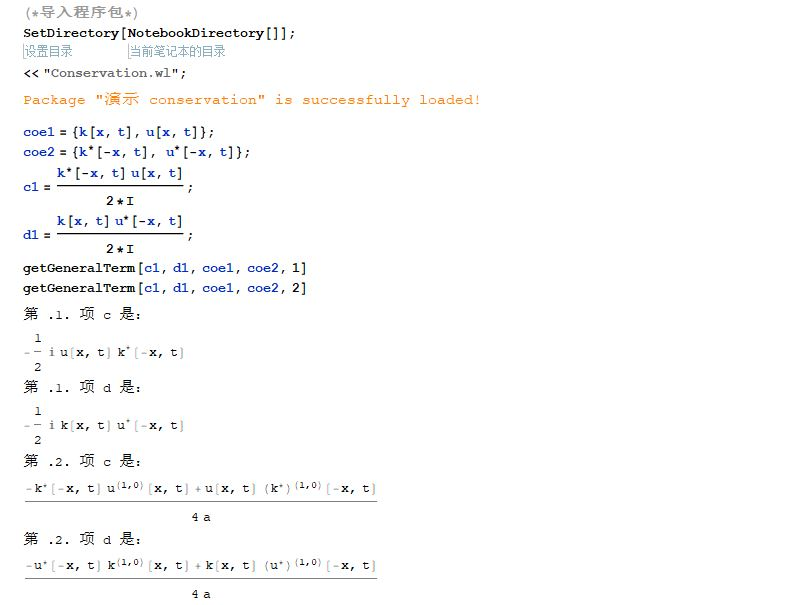
\includegraphics[width=0.97\linewidth]{getGeneralTerm.jpg}
	\caption{求解依赖项的运行结果}
	%with same parameters~$k=1 , \alpha_2(t)=1, \alpha_0(t)=0$.
	\label{picture-5-1}
\end{figure}
下面是对程序的使用过程的介绍:如果想要使用该程序,首先导入封装该函数的程序包 $Conservation.wl$,以 .wl 为后缀的文件是 Mathematica 所提供的自定义程序包的文件格式。如果加载程序包后出现 $Package \ "Conservation" \ is \ successfully \  loaded!$ 的输出语句说明程序包加载成功。然后就可以调用程序包中的函数,运行结果如图 \ref{picture-5-1} 所示。该图只展示了所得到$c_n, d_n$ 前两项的结果。可以看到,图 \ref{picture-5-1} 的运行结果和第四章第三节中得到的结果是一致的。


\subsection{守恒律求解的实现}
在实现依赖项求解之后,接下来的问题就是如何求解方程的守恒律。和上一小节的过程类似,我们在得到方程守恒律的通项公式后,就可以很容易的求得任意项的守恒律,这些通项公式中的一些参数系数部分是上一小节求得的结果,另一部分是固定形式的参数,它们被当作变量传入到代码的函数中。

以下是函数的简单实现
\begin{lstlisting}[language=Mathematica,caption=守恒律求解的实现]
(*
	clist: 通项公式 cn 的前 n 项列表
	dlist: 通项公式 dn 的前 n 项列表
	coe1: 对应系数的函数列表
	coe2: 对应系数的函数其它形式(例如共轭)列表
	n: 表示第 n 组的结果
*)
Conservation[clist_, dlist_, coe1_, coe2_, n_]:=Module[{Dlist, Flist, dn, fn},
	If[n <= 0, Print["n 输入不合法"],
	If[Length[coe1]!= Length[coe2] || Length[clist] != Length[dlist],
	Print["系数列表长度不符合要求"],
	
	(*守恒律 Dn 的列表*)
	Dlist = List[];
	(*守恒律 Fn 的列表*)
	Flist = List[];
	(*列表 Dlist, Flist 的首项内容*)
	Dlist = Append[Dlist, 0];
	Flist = Append[Flist, 0];

	For[i=1, i <= n, i++,
	dn = a(coe1[[1]]coe2[[2]] clist[[n+1]] + coe2[[1]]coe1[[2]] dlist[[n+1]]);
	fn = b[t](coe1[[3]] coe1[[1]] clist[[n+2]] + coe1[[4]] coe1[[1]] clist[[n+1]] +  2/3 coe1[[1]]coe2[[2]] clist[[n+3]]+  2/3 coe1[[2]]coe2[[1]] dlist[[n+3]]-coe2[[3]] coe2[[1]] dlist[[n+2]]+coe2[[4]] coe2[[1]]dlist[[n+1]]);
	Dlist = Append[Dlist, dn];
	Flist = Append[Flist, fn];
	]
	Print["第 ".n." 项 D 是:"]
	Print[Expand[Dlist[[n+1]]]];
	Print["第 ".n." 项 F 是:"]
	Print[Expand[Flist[[n+1]]]];
]
]
]

\end{lstlisting}
上述代码中 $Conservation$ 函数接收五个参数,$clist$ 是上一小节得到的 $c_n$ 前 $n$ 项的列表,而$dlist$ 是则是上一小节中的得到的 $d_n$ 的前 $n$ 项列表,$coe1$ 表示对应系数的函数列表,$co2$ 对应系数的函数其它形式列表,一般情况下是共轭形式,$n$ 表示想要得到第几组守恒律。程序的内部过程是关于 Sasa-Satsuma 类型方程的守恒律的求解过程。其中守恒律中的 $D_n$ 和 $F_n$ 项的表达式如下所示,
\begin{align}
  & D_{n} = a(ku^{*}c_{n} + k^{*}ud_{n}) \\
  & F_{n} = b(t)\left[A_{2}kc_{n+1} + A_{4}kc_{n} + \frac{2}{3}ku^{*}c_{n+2} + \frac{2}{3}uk^{*}d_{n+2} - A_{2}^{*}k^{*}d_{n+1} + A_{4}^{*}k^{*}d_{n}\right]
\end{align}
对于 Sasa-Satsuma 类型的方程守恒律的求解基本上都可以通过上述的方程来求得,因此只要指导表达式中对应元素的形式就能求得其中任意组的守恒律。而表达式中的元素 $A_2, A_4, k$ 等根据方程的不同可能会有不同的形式,$c_n, d_n$ 的形式相对固定,并且求解过程在上一小节中已给出。下面介绍该函数的使用过程和运行结果。

使用上述代码之前需要调用上一小节中的代码。以本论文中的第四章研究的方程 (\ref{nss-1}) 为例,运用上述函数求得方程 (\ref{nss-1}) 的守恒律:首先导入封装该函数的程序包 $Conservation.wl$,加载程序包后出现 $Package \ "Conservation" \ is \ successfully \  loaded!$ 表示加载成功。然后就可以调用程序包中的 $getGeneralTerm$ 函数,并在该函数的内部调用 $Conservation$,并传入相应的参数。运行结果如图 \ref{picture-5-2} 所示。这里我们只运行给出了方程 (\ref{nss-1}) 的第一组守恒律的结果。可以看到守恒律的结果和第四章第三节中的结果是一致的。
\begin{figure}[!htp]
\centering
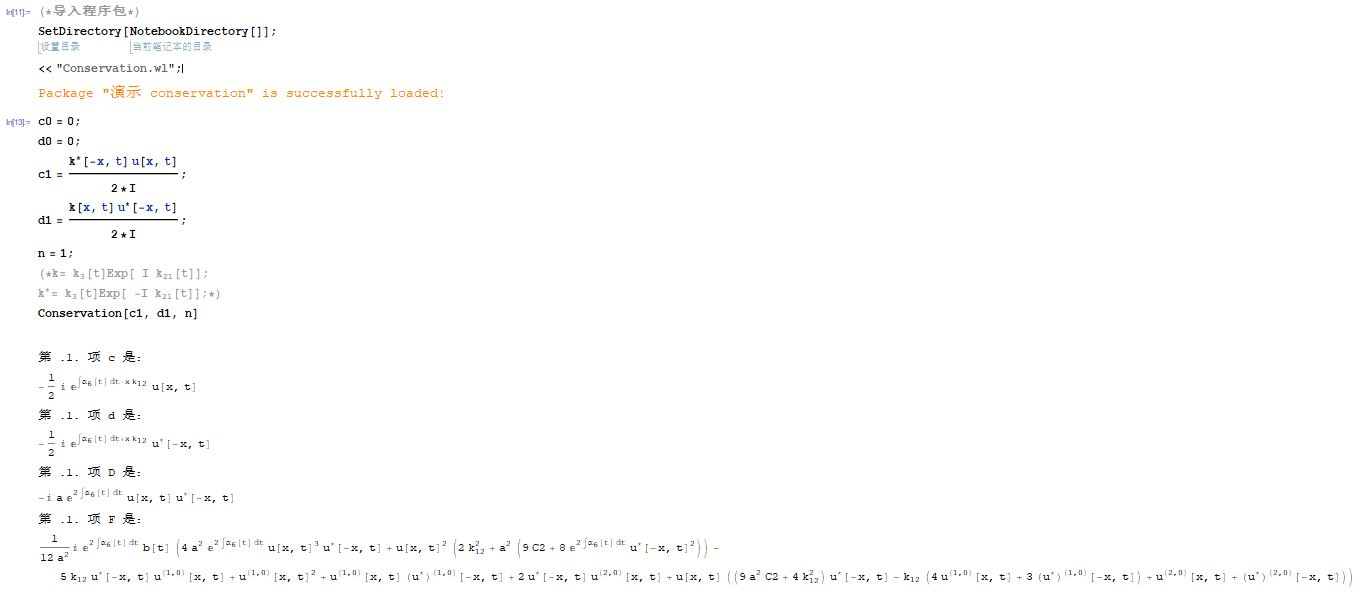
\includegraphics[width=\linewidth]{getConservation.jpg}
\caption{求解方程的守恒律}
%with same parameters~$k=1 , \alpha_2(t)=1, \alpha_0(t)=0$.
\label{picture-5-2}
\end{figure}

\section{验证守恒律}
上一节实现了用于求解方程守恒律的程序,接下来这一节对得到的守恒律进行验证,然而不像求解守恒律那么般有规律,不同组的守恒律验证往往又不一样,因此目前程序只对前两组守恒律进行验证。

\begin{lstlisting}[language=Mathematica,caption=验证守恒律]
(*
	equ1: 表示多研究的目标方程
	equ2: 表示目标方程的共轭形式
	d, f: 表示守恒律的表达式
	u, v: 表示方程中的原子函数和其共轭函数
	n: 表示第几组守恒律
	c: 表示一个常数项
*)
validateConservation[equ1_, equ2_, u_, v_, d_, f_, n_, c_]:=Module[{result},
	If[n != 1 && n != 2, Print["n 输入不合法"],
	
	result = 0;

	If[n == 1,
		result = Simplify[(D[d,t] - D[f, x]) / (v * equ1 - u * equ2) / c];
	];
	If[n == 2,
		result = Simplify[(D[d,t] - D[f, x])/(D[equ2, x] * u -D[equ1, x] * v + D[v, x] * equ1 + D[u, x] * equ2) / c];
	];
	Print["结果为". result];
	If[result == 1,
		Print["验证成功"],
		Print["验证失败"]
	];
	]
];
\end{lstlisting}
$validateConservation$ 函数接收 8 个参数, $equ1, equ2$ 分别表示所研究的目标方程和目标方程的共轭形式,$u, v$ 分别是方程中的原子函数及其的共轭函数,即 $equ1, equ2$ 都是关于函数 $u, v$ 的非线性偏微分方程。$d, f$ 是前一步中求得的一组守恒律。$n$ 表示传入进来的守恒律是第几组,$c$ 表示一个不含函数 $u[x,t]$ 和其共轭函数的常数项。验证的思路如下:将守恒律中 $d$ 项函数对 $t$ 进行求导,对守恒律中 $f$ 项函数对 $x$ 求导,两者的结果相减,如果结果等于 0,那么守恒律就成立。但是一般相减后结果仍然是一个关于函数 $u$ 的多项式,如果它能与研究的目标方程等价,那么结果也就自然等于 0 了。这时,往往对原方程和其共轭方程进行各种形式的变形,使其能够与之前相减的结果等价。对于不同组的守恒律找到的变形往往是不同的,越是往后的守恒律往往形式越是复杂,因此该程序目前是能验证守恒律中前两组相对简单的形式。验证的结果如图  \ref{picture-5-3} 所示,从图中的运行结果我们可以看到方程的前两组的守恒律都成立。

\begin{figure}[!htp]
	\centering
	\subfigure[验证第一组守恒律成立]{
		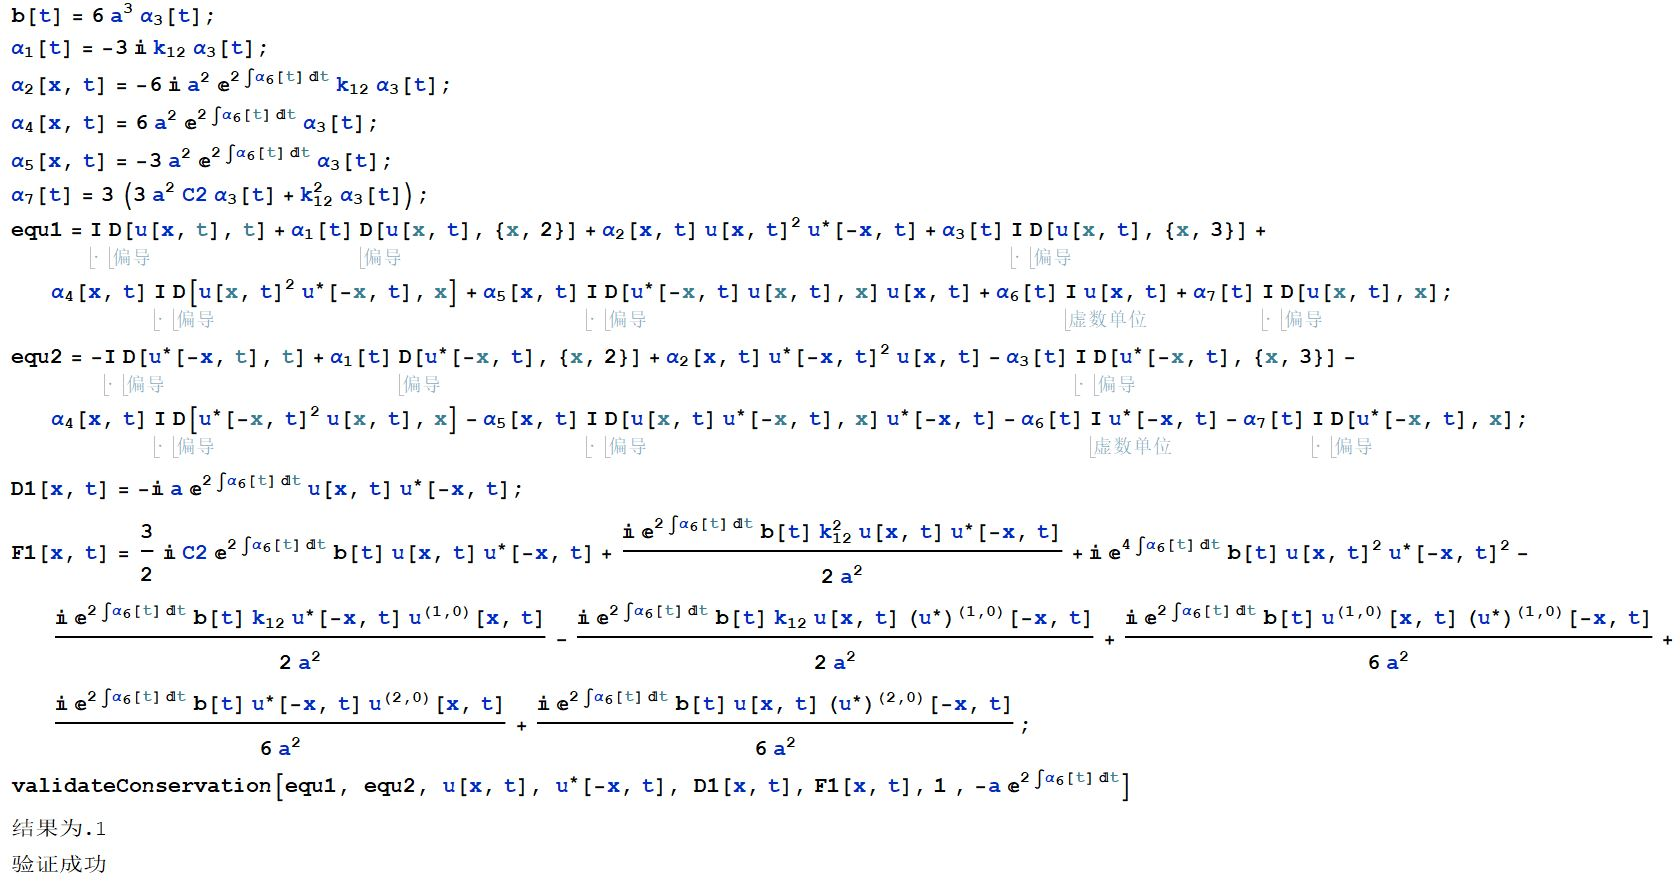
\includegraphics[width=\linewidth]{validateConservation1.jpg}
		\label{picture-5-31}
	}
	\ \
	\subfigure[验证第二组守恒律成立]{
		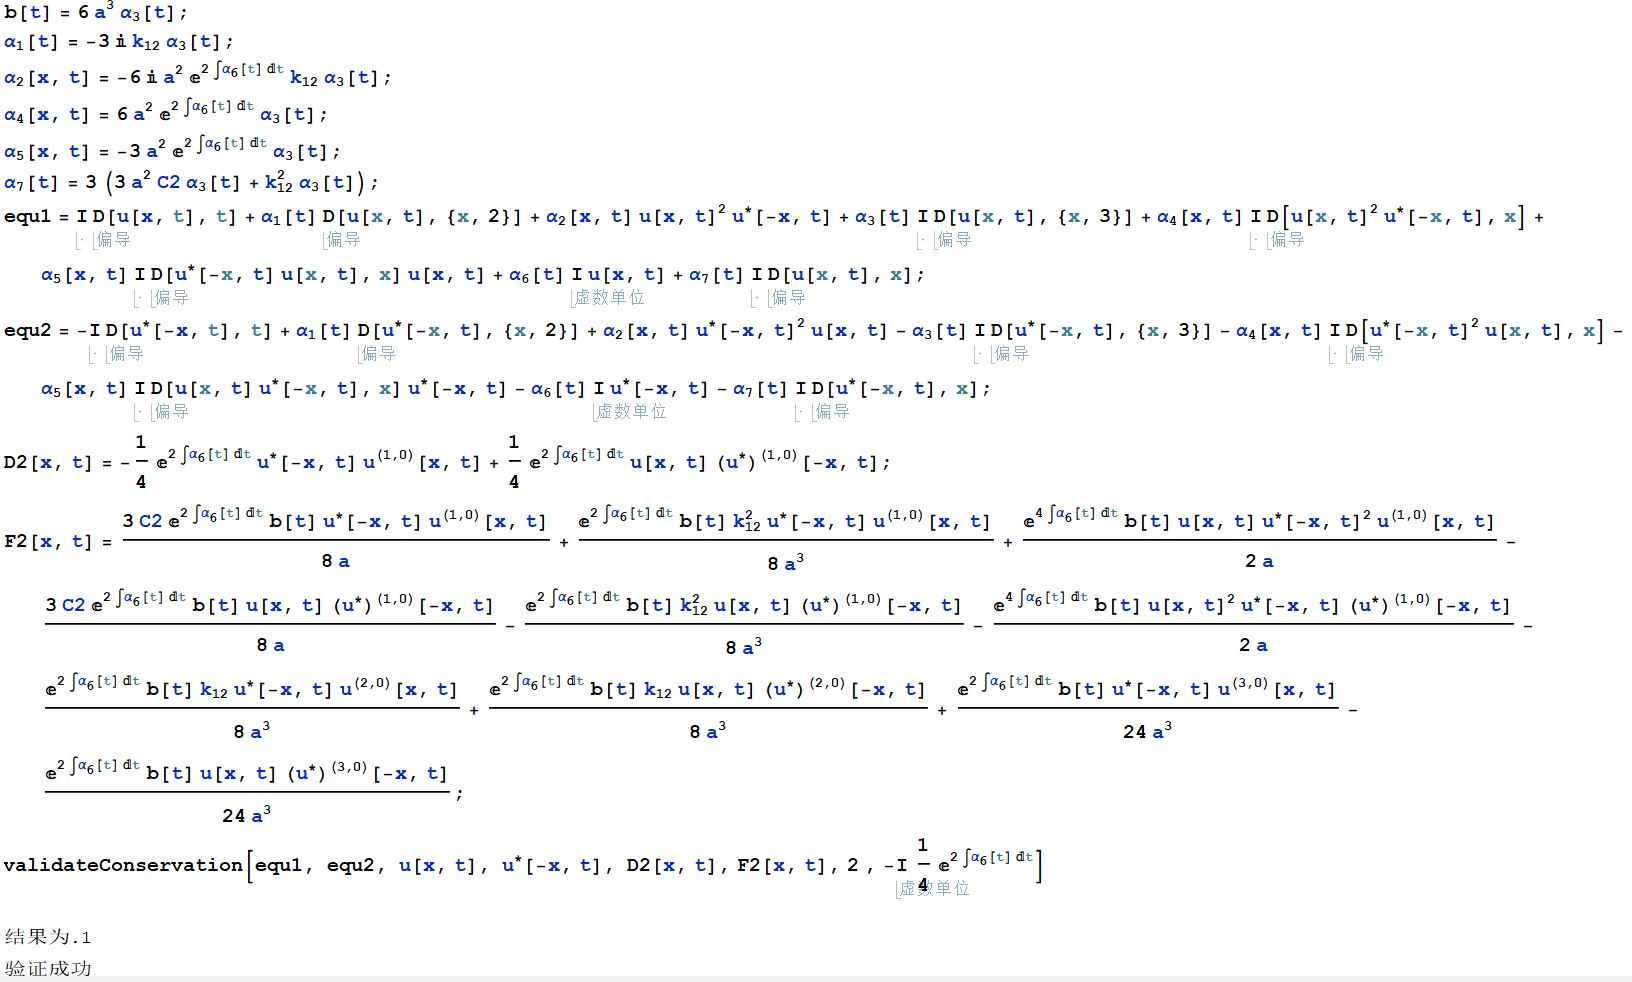
\includegraphics[width=\linewidth]{validateConservation2.jpg}
		\label{picture-5-32}
	}
    \caption{验证守恒律成立}
	\label{picture-5-3}
\end{figure}



\section{本章小结}
本章首先介绍了符号计算软件 Mathematica 的程序编程语言 Wolfram 的基本语法和常用的函数,然后基于 Mathematica 开发了用于得到 ss 方程的守恒律的程序包。这个程序包主要包含两部分的内容,首先是根据方程无穷守恒律的关系表达式迭代推导出前几组的守恒律具体的形式,即 $Conservation$ 函数的实现内容;然后,根据之前得到的守恒律进行验证,验证的方法就是通过寻找方程的各种变形使守恒律达到平衡,即 $validateConservation$ 函数的具体实现内容。最后可以看到本章通过程序包求得的守恒律与第四章求得的守恒律完全一致,并最终通过了验证,这也说明程序包运行的具有较好的正确性和可靠性。


\end{CJK}
\end{document}
